% Generated fragments require trusted human review before compilation.
% This binder never requests shell escape or runs external tools.
\documentclass[11pt]{article}
% Trusted shared apparatus. Requires LuaLaTeX; never use shell escape.
\usepackage{fontspec}
\defaultfontfeatures{Ligatures=TeX}
\IfFontExistsTF{Noto Serif}{\setmainfont{Noto Serif}}{%
  \IfFontExistsTF{DejaVu Serif}{\setmainfont{DejaVu Serif}}{%
    \IfFontExistsTF{Times New Roman}{\setmainfont{Times New Roman}}{%
      \PackageError{gelfand-binder}{No configured Cyrillic serif font installed}{Install Noto Serif or DejaVu Serif, or select an installed Cyrillic font.}%
    }%
  }%
}
\IfFontExistsTF{Noto Sans}{\setsansfont{Noto Sans}}{%
  \IfFontExistsTF{DejaVu Sans}{\setsansfont{DejaVu Sans}}{\setsansfont{Arial}}%
}
\IfFontExistsTF{Noto Sans Mono}{\setmonofont{Noto Sans Mono}}{%
  \IfFontExistsTF{DejaVu Sans Mono}{\setmonofont{DejaVu Sans Mono}}{\setmonofont{Courier New}}%
}
\usepackage[a4paper,margin=22mm]{geometry}
\usepackage{amsmath,amssymb,amsthm,mathtools}
\usepackage{xcolor}
\usepackage{tikz}
\usepackage{tikz-cd}
\usetikzlibrary{arrows.meta,positioning,calc}
\usepackage{hyperref}
\hypersetup{unicode=true,colorlinks=true,linkcolor=blue,pdftitle={Gelfand transcription binder}}
\newtheorem{theorem}{Theorem}
\newtheorem{lemma}{Lemma}
\newtheorem{proposition}{Proposition}
\newtheorem{corollary}{Corollary}
\theoremstyle{definition}
\newtheorem{definition}{Definition}
\newtheorem{example}{Example}
\theoremstyle{remark}
\newtheorem{remark}{Remark}
\setlength{\parindent}{0pt}
\setlength{\parskip}{0.55em}
\setlength{\emergencystretch}{3em}
\newcommand{\SourcePage}[2]{%
  \clearpage\phantomsection\label{#1:source-page}%
  \addcontentsline{toc}{subsection}{#1}%
  {\small\sffamily\color{blue!60!black}Source scan frame: #1; visible page/leaf label: #2}\par\medskip%
}
\newcommand{\Unclear}[3]{%
  \begingroup\color{orange!70!black}%
  [Unresolved reading #1/#2: #3]\endgroup%
}
\newcommand{\Incomplete}[3]{%
  \par\begingroup\color{red!65!black}\textbf{Incomplete #1/#2:} #3\endgroup\par%
}
\newcommand{\SourceFigure}[3]{%
  \par\begingroup\color{blue!60!black}\textbf{\hyperref[#1:source-page]{Source figure #1/#2}:} #3%
  \par\textit{Consult the authoritative scan at this locator.}\endgroup\par%
}



% Reader layout only. Original diplomatic text is retained verbatim.
\setlength{\parskip}{0.35em}
\setlength{\emergencystretch}{4em}
\renewcommand{\SourcePage}[2]{%
  \par\addvspace{1em}\phantomsection\label{#1:source-page}%
  \addcontentsline{toc}{subsection}{#1}%
  {\footnotesize\sffamily\color{blue!55!black}#1%
    \def\givenlabel{#2}\def\nolabel{unlabelled}%
    \ifx\givenlabel\nolabel\else\quad[номер в источнике: #2]\fi
  }\par\nobreak\smallskip%
}
\renewcommand{\Unclear}[3]{%
  \begingroup\color{orange!65!black}%
  \ifmmode\text{[неясно: #3]}\else[неясно: #3]\fi\endgroup%
}
\renewcommand{\Incomplete}[3]{%
  \par\begingroup\color{red!60!black}\textbf{Неразобранный фрагмент:} #3%
  \endgroup\par%
}
\renewcommand{\SourceFigure}[3]{%
  \par\begingroup\color{blue!55!black}\textbf{Рисунок:} #3%
  \par{\small\textit{Исходный рисунок: \hyperref[#1:source-page]{#1}, #2.}}%
  \endgroup\par%
}
\hypersetup{pdftitle={Семинар И. М. Гельфанда. Дипломатическая транскрипция},pdfauthor={},pdfsubject={Русское рабочее издание с отмеченными сомнительными чтениями}}

\usepackage[normalem]{ulem}
\usepackage{newunicodechar}
\usepackage{adjustbox}
\newfontfamily\SourceSymbolFont{Segoe UI Symbol}
\newfontfamily\SourceCJKFont{MS Gothic}
\let\DiplomaticMathUnderline\underline
\renewcommand{\underline}[1]{\ifmmode\DiplomaticMathUnderline{#1}\else\uline{#1}\fi}
\newunicodechar{→}{\ifmmode\text{{\SourceSymbolFont\char"2192}}\else{\SourceSymbolFont\char"2192}\fi}
\newunicodechar{⇒}{\ifmmode\text{{\SourceSymbolFont\char"21D2}}\else{\SourceSymbolFont\char"21D2}\fi}
\newunicodechar{∀}{\ifmmode\text{{\SourceSymbolFont\char"2200}}\else{\SourceSymbolFont\char"2200}\fi}
\newunicodechar{∂}{\ifmmode\text{{\SourceSymbolFont\char"2202}}\else{\SourceSymbolFont\char"2202}\fi}
\newunicodechar{∈}{\ifmmode\text{{\SourceSymbolFont\char"2208}}\else{\SourceSymbolFont\char"2208}\fi}
\newunicodechar{∌}{\ifmmode\text{{\SourceSymbolFont\char"220C}}\else{\SourceSymbolFont\char"220C}\fi}
\newunicodechar{√}{\ifmmode\text{{\SourceSymbolFont\char"221A}}\else{\SourceSymbolFont\char"221A}\fi}
\newunicodechar{∞}{\ifmmode\text{{\SourceSymbolFont\char"221E}}\else{\SourceSymbolFont\char"221E}\fi}
\newunicodechar{∧}{\ifmmode\text{{\SourceSymbolFont\char"2227}}\else{\SourceSymbolFont\char"2227}\fi}
\newunicodechar{∩}{\ifmmode\text{{\SourceSymbolFont\char"2229}}\else{\SourceSymbolFont\char"2229}\fi}
\newunicodechar{∪}{\ifmmode\text{{\SourceSymbolFont\char"222A}}\else{\SourceSymbolFont\char"222A}\fi}
\newunicodechar{∫}{\ifmmode\text{{\SourceSymbolFont\char"222B}}\else{\SourceSymbolFont\char"222B}\fi}
\newunicodechar{∴}{\ifmmode\text{{\SourceSymbolFont\char"2234}}\else{\SourceSymbolFont\char"2234}\fi}
\newunicodechar{∼}{\ifmmode\text{{\SourceSymbolFont\char"223C}}\else{\SourceSymbolFont\char"223C}\fi}
\newunicodechar{≈}{\ifmmode\text{{\SourceSymbolFont\char"2248}}\else{\SourceSymbolFont\char"2248}\fi}
\newunicodechar{≠}{\ifmmode\text{{\SourceSymbolFont\char"2260}}\else{\SourceSymbolFont\char"2260}\fi}
\newunicodechar{≤}{\ifmmode\text{{\SourceSymbolFont\char"2264}}\else{\SourceSymbolFont\char"2264}\fi}
\newunicodechar{≥}{\ifmmode\text{{\SourceSymbolFont\char"2265}}\else{\SourceSymbolFont\char"2265}\fi}
\newunicodechar{⊕}{\ifmmode\text{{\SourceSymbolFont\char"2295}}\else{\SourceSymbolFont\char"2295}\fi}
\newunicodechar{⊗}{\ifmmode\text{{\SourceSymbolFont\char"2297}}\else{\SourceSymbolFont\char"2297}\fi}
\newunicodechar{①}{\ifmmode\text{{\SourceSymbolFont\char"2460}}\else{\SourceSymbolFont\char"2460}\fi}
\newunicodechar{②}{\ifmmode\text{{\SourceSymbolFont\char"2461}}\else{\SourceSymbolFont\char"2461}\fi}
\newunicodechar{③}{\ifmmode\text{{\SourceSymbolFont\char"2462}}\else{\SourceSymbolFont\char"2462}\fi}
\newunicodechar{④}{\ifmmode\text{{\SourceSymbolFont\char"2463}}\else{\SourceSymbolFont\char"2463}\fi}
\newunicodechar{Ⓗ}{\ifmmode\text{{\SourceSymbolFont\char"24BD}}\else{\SourceSymbolFont\char"24BD}\fi}
\newunicodechar{〃}{\ifmmode\text{{\SourceCJKFont\char"3003}}\else{\SourceCJKFont\char"3003}\fi}


% Reader revision 3. Annotation wording and candidates remain unchanged.
\setmainfont{NotoSerif-Regular.ttf}[Path=C:/Windows/Fonts/,ItalicFont=NotoSerif-Italic.ttf,BoldFont=NotoSerif-Bold.ttf,BoldItalicFont=NotoSerif-BoldItalic.ttf]
\usetikzlibrary{shapes.geometric,decorations.pathreplacing,decorations.markings,patterns,fit}
\newsavebox{\ReaderAnnotationBox}
\newcommand{\ReaderAnnotation}[1]{%
  \sbox{\ReaderAnnotationBox}{[неясно: #1]}%
  \ifdim\wd\ReaderAnnotationBox>.70\linewidth
    \parbox[t]{.70\linewidth}{\raggedright[неясно: #1]}%
  \else\usebox{\ReaderAnnotationBox}\fi%
}
\ExplSyntaxOn
\cs_new_protected:Npn \reader_unclear_candidate:n #1
 {
  \tl_set:Nx \l_tmpa_tl { \tl_to_str:n {#1} }
  % Text explicitly guarded inside a mathematical candidate remains math-safe.
  \regex_replace_all:nnN { \\(?:text|textrm|textnormal|textbf|operatorname)\s*\{[^{}]*\} } { } \l_tmpa_tl
  \regex_match:nVTF { [\x{0400}-\x{052F}] | \$ } \l_tmpa_tl
   { \ifmmode \text{\ReaderAnnotation{#1}} \else \ReaderAnnotation{#1} \fi }
   {
    \ifmmode
      [\text{неясно:~}#1]
    \else
      \regex_match:nVTF { [_^] | \\ } \l_tmpa_tl
       { \ensuremath{[\text{неясно:~}#1]} }
       { \ReaderAnnotation{#1} }
    \fi
   }
 }
\RenewDocumentCommand \Unclear { m m m }
 { \begingroup\color{orange!65!black}\reader_unclear_candidate:n{#3}\endgroup }
\ExplSyntaxOff
\newsavebox{\ReaderIncompleteBox}
\newcommand{\ReaderIncompleteNote}[1]{%
 \sbox{\ReaderIncompleteBox}{\textbf{Неразобранный фрагмент:} #1}%
 \ifdim\wd\ReaderIncompleteBox>.70\linewidth
  \parbox[t]{.70\linewidth}{\raggedright\textbf{Неразобранный фрагмент:} #1}%
 \else\usebox{\ReaderIncompleteBox}\fi%
}
\renewcommand{\Incomplete}[3]{%
 \ifmmode\text{\color{red!60!black}\ReaderIncompleteNote{#3}}%
 \else\leavevmode\begingroup\color{red!60!black}\ReaderIncompleteNote{#3}\endgroup\fi%
}
% Ragged right avoids stretching long untranslated abbreviations into margins.
\AtBeginDocument{\raggedright}
\newunicodechar{А}{\ifmmode\text{\char"410\relax}\else\char"410\relax\fi}
\newunicodechar{Б}{\ifmmode\text{\char"411\relax}\else\char"411\relax\fi}
\newunicodechar{В}{\ifmmode\text{\char"412\relax}\else\char"412\relax\fi}
\newunicodechar{Г}{\ifmmode\text{\char"413\relax}\else\char"413\relax\fi}
\newunicodechar{Д}{\ifmmode\text{\char"414\relax}\else\char"414\relax\fi}
\newunicodechar{Е}{\ifmmode\text{\char"415\relax}\else\char"415\relax\fi}
\newunicodechar{Ж}{\ifmmode\text{\char"416\relax}\else\char"416\relax\fi}
\newunicodechar{З}{\ifmmode\text{\char"417\relax}\else\char"417\relax\fi}
\newunicodechar{И}{\ifmmode\text{\char"418\relax}\else\char"418\relax\fi}
\newunicodechar{Й}{\ifmmode\text{\char"419\relax}\else\char"419\relax\fi}
\newunicodechar{К}{\ifmmode\text{\char"41A\relax}\else\char"41A\relax\fi}
\newunicodechar{Л}{\ifmmode\text{\char"41B\relax}\else\char"41B\relax\fi}
\newunicodechar{М}{\ifmmode\text{\char"41C\relax}\else\char"41C\relax\fi}
\newunicodechar{Н}{\ifmmode\text{\char"41D\relax}\else\char"41D\relax\fi}
\newunicodechar{О}{\ifmmode\text{\char"41E\relax}\else\char"41E\relax\fi}
\newunicodechar{П}{\ifmmode\text{\char"41F\relax}\else\char"41F\relax\fi}
\newunicodechar{Р}{\ifmmode\text{\char"420\relax}\else\char"420\relax\fi}
\newunicodechar{С}{\ifmmode\text{\char"421\relax}\else\char"421\relax\fi}
\newunicodechar{Т}{\ifmmode\text{\char"422\relax}\else\char"422\relax\fi}
\newunicodechar{У}{\ifmmode\text{\char"423\relax}\else\char"423\relax\fi}
\newunicodechar{Ф}{\ifmmode\text{\char"424\relax}\else\char"424\relax\fi}
\newunicodechar{Х}{\ifmmode\text{\char"425\relax}\else\char"425\relax\fi}
\newunicodechar{Ц}{\ifmmode\text{\char"426\relax}\else\char"426\relax\fi}
\newunicodechar{Ч}{\ifmmode\text{\char"427\relax}\else\char"427\relax\fi}
\newunicodechar{Ш}{\ifmmode\text{\char"428\relax}\else\char"428\relax\fi}
\newunicodechar{Щ}{\ifmmode\text{\char"429\relax}\else\char"429\relax\fi}
\newunicodechar{Ъ}{\ifmmode\text{\char"42A\relax}\else\char"42A\relax\fi}
\newunicodechar{Ы}{\ifmmode\text{\char"42B\relax}\else\char"42B\relax\fi}
\newunicodechar{Ь}{\ifmmode\text{\char"42C\relax}\else\char"42C\relax\fi}
\newunicodechar{Э}{\ifmmode\text{\char"42D\relax}\else\char"42D\relax\fi}
\newunicodechar{Ю}{\ifmmode\text{\char"42E\relax}\else\char"42E\relax\fi}
\newunicodechar{Я}{\ifmmode\text{\char"42F\relax}\else\char"42F\relax\fi}
\newunicodechar{а}{\ifmmode\text{\char"430\relax}\else\char"430\relax\fi}
\newunicodechar{б}{\ifmmode\text{\char"431\relax}\else\char"431\relax\fi}
\newunicodechar{в}{\ifmmode\text{\char"432\relax}\else\char"432\relax\fi}
\newunicodechar{г}{\ifmmode\text{\char"433\relax}\else\char"433\relax\fi}
\newunicodechar{д}{\ifmmode\text{\char"434\relax}\else\char"434\relax\fi}
\newunicodechar{е}{\ifmmode\text{\char"435\relax}\else\char"435\relax\fi}
\newunicodechar{ж}{\ifmmode\text{\char"436\relax}\else\char"436\relax\fi}
\newunicodechar{з}{\ifmmode\text{\char"437\relax}\else\char"437\relax\fi}
\newunicodechar{и}{\ifmmode\text{\char"438\relax}\else\char"438\relax\fi}
\newunicodechar{й}{\ifmmode\text{\char"439\relax}\else\char"439\relax\fi}
\newunicodechar{к}{\ifmmode\text{\char"43A\relax}\else\char"43A\relax\fi}
\newunicodechar{л}{\ifmmode\text{\char"43B\relax}\else\char"43B\relax\fi}
\newunicodechar{м}{\ifmmode\text{\char"43C\relax}\else\char"43C\relax\fi}
\newunicodechar{н}{\ifmmode\text{\char"43D\relax}\else\char"43D\relax\fi}
\newunicodechar{о}{\ifmmode\text{\char"43E\relax}\else\char"43E\relax\fi}
\newunicodechar{п}{\ifmmode\text{\char"43F\relax}\else\char"43F\relax\fi}
\newunicodechar{р}{\ifmmode\text{\char"440\relax}\else\char"440\relax\fi}
\newunicodechar{с}{\ifmmode\text{\char"441\relax}\else\char"441\relax\fi}
\newunicodechar{т}{\ifmmode\text{\char"442\relax}\else\char"442\relax\fi}
\newunicodechar{у}{\ifmmode\text{\char"443\relax}\else\char"443\relax\fi}
\newunicodechar{ф}{\ifmmode\text{\char"444\relax}\else\char"444\relax\fi}
\newunicodechar{х}{\ifmmode\text{\char"445\relax}\else\char"445\relax\fi}
\newunicodechar{ц}{\ifmmode\text{\char"446\relax}\else\char"446\relax\fi}
\newunicodechar{ч}{\ifmmode\text{\char"447\relax}\else\char"447\relax\fi}
\newunicodechar{ш}{\ifmmode\text{\char"448\relax}\else\char"448\relax\fi}
\newunicodechar{щ}{\ifmmode\text{\char"449\relax}\else\char"449\relax\fi}
\newunicodechar{ъ}{\ifmmode\text{\char"44A\relax}\else\char"44A\relax\fi}
\newunicodechar{ы}{\ifmmode\text{\char"44B\relax}\else\char"44B\relax\fi}
\newunicodechar{ь}{\ifmmode\text{\char"44C\relax}\else\char"44C\relax\fi}
\newunicodechar{э}{\ifmmode\text{\char"44D\relax}\else\char"44D\relax\fi}
\newunicodechar{ю}{\ifmmode\text{\char"44E\relax}\else\char"44E\relax\fi}
\newunicodechar{я}{\ifmmode\text{\char"44F\relax}\else\char"44F\relax\fi}
\newunicodechar{Ё}{\ifmmode\text{\char"401\relax}\else\char"401\relax\fi}
\newunicodechar{ё}{\ifmmode\text{\char"451\relax}\else\char"451\relax\fi}

\newunicodechar{æ}{\ifmmode\text{\char"E6\relax}\else\char"E6\relax\fi}
\newunicodechar{−}{\ifmmode\mathbin{\text{\SourceSymbolFont\char"2212\relax}}\else{\SourceSymbolFont\char"2212\relax}\fi}

\begin{document}
\begin{center}
{\Large Семинар И. М. Гельфанда}\par\medskip
{\LARGE Дипломатическая транскрипция}\par\bigskip
{\large Рабочее русское издание}\par\medskip
{\large Том 28 из 34. Архивная глава 028}\par\bigskip
Кадры GELFAND-P001253 -- GELFAND-P001296\par

\end{center}
\medskip
Сокращения, отменённые записи и сомнительные чтения сохранены.
Неразобранные фрагменты отмечены в тексте. Математические утверждения
источника переданы без молчаливых исправлений.

Это рабочее издание: сверка с рукописью продолжается. В текущем комплекте
учтены 1503 из 1527 кадров; 24 кадра пока представлены явными указателями
отсутствующего возврата. Полный журнал чтений и происхождения данных
сохранён в основном рабочем переплёте.

Границы кадров показаны небольшими синими указателями; печатный текст
продолжается без обязательного разрыва страницы после каждого кадра.
\bigskip\hrule\bigskip
\SourcePage{GELFAND-P001253}{unlabelled}
\noindent\underline{\underline{17/II — 86 г.}}\qquad\underline{Сем. Гельфанда.}

\noindent\underline{\underline{Бейлинсон А.}}\qquad
[Зачёркнуто: \Unclear{GELFAND-P001253}{title-cancel}{О … [возможно: «О теории»].}]
\underline{Детерминант Квиллена, струны и пр.}

Вычисляем статсумму
\begin{equation*}
Z=\sum_{p\geq0}Z_p .\tag{1}
\end{equation*}
\noindent $p$ — род
\begin{equation*}
Z_p=\int_{M_p}\mu_p,\qquad
\begin{aligned}
M_p&\text{ — пр-во модулей кривых рода }p.\\
\mu_p&\text{ — естеств. возник. мера}
\end{aligned}\tag{2}
\end{equation*}
При $p=1$ независимо вычислили Кронекер (1890) и Шапиро (1972)
(одинаково)
\begin{equation*}
\mu_1=\left|\frac{dq}{q}\right|^2\Delta(q)^{-2}\log|q|^{-13},
\qquad \Delta(q)=q\prod(1-q^n)^{24}.\tag{3}
\end{equation*}
[В показателе после $\log|q|$ густая правка;
\Unclear{GELFAND-P001253}{log-exponent}{читается $-13$; выше приписано $13$ и неразборчивая запись в скобках, от неё стрелка к показателю.}]

$\mu_1$ — мера на пр-ве модулей элл. кривых

\begin{center}— . —\end{center}
$X$ — пов. рода $p$; $g$ — метрика на $X$;
$L$ — одномерное голом. рассл. на $X$
(голом. структ., индуц. метрикой), $h$ — эрмитова метрика на $L$
\begin{equation*}
\bar\partial:\Gamma(L)\longrightarrow\Gamma(L\otimes\Omega^{0,1}).\tag{4}
\end{equation*}
Тогда
\begin{equation*}
\underset{\substack{|\\\text{голом. сечения}}}{H^0(X,L)}
=\operatorname{Ker}\bar\partial,\qquad
H^1(X,L)=\operatorname{Coker}\bar\partial=\operatorname{Ker}\bar\partial^{+}.
\tag{5}
\end{equation*}
(Голом. рассл. описываются одним дискр. пар. — числом Черна и $p$
непрерывными пар. — точка на якобиане)

$H^0$, $H^1$ конечномерны
\begin{equation*}
d(X,L):=\frac{\det H^0(X,L)}{\det H^1(X,L)}.\tag{6}
\end{equation*}
$\det H^0=\max$ внешн. степень $H^0$ — одномерное вект. пр-во

[Следующая строка обозначена длинными чертами и знаком повтора;
в ней вместо $H^0$ стоит $H^1$.]

Поэтому $d(X,L)$ — тоже 1-мерное вект. пр-во.
(ф-ии на $\det H^1$ со знач. в $\det H^0$)

На нём есть естеств. метрика
\begin{equation*}
\begin{array}{l|l}
e_1,\ldots,e_k\text{ — базис в }H^0&
\displaystyle d(X,L)\ni
\underset{\substack{\uparrow\\\mathbb C}}{\lambda}
\frac{e_1\wedge\cdots\wedge e_k}{g_1\wedge\cdots\wedge g_d}\\
g_1,\ldots,g_d\text{ — базис в }H^1&
\end{array}
\end{equation*}

\SourcePage{GELFAND-P001254}{4}
Метрика будет опр. в 2 этапа.

Сначала \underline{глупая} метрика.
Рассм. [вписано сверху: естеств.] метрику на
[зачёркнуто: \Unclear{GELFAND-P001254}{top-cancel}{пр. [неуверенно].}]
$\Gamma(L)$ и на $\Omega^{0,1}$,
определяющие там предгильбертовы структуры.

На $H^0$ и $H^1=\operatorname{Ker}\bar\partial^{+}$ тоже индуцируются метрики
$\Rightarrow$\newline
$\Rightarrow$ возникает метрика в $d(X,L)$, называемая глупой.

[Вписано сверху: Построим.] \underline{Правильную метрику.}
[Слева стрелка вниз.]

Рассм. $\Delta=\bar\partial^{+}\bar\partial$ и его $\det\Delta$,
вычисленный Белавиным и Книжником;

$\Delta'$ — тот же $\Delta$, но с выброшенными нулевыми модами.
\begin{equation*}
\det\Delta'=\exp\bigl(-\zeta'_{\Delta'}(0)\bigr),
\end{equation*}
\begin{equation*}
\zeta_{\Delta'}(s)=
\sum_{\substack{\lambda\in\text{соб. зн.}\,\Delta,\\\lambda\ne0}}
\lambda^{-s},\qquad\operatorname{Re}s>1
\end{equation*}
\begin{equation*}
\begin{aligned}
&\underline{\text{Метрика Квиллена на }d(X,L)}
\quad\left(\text{из статьи в ФА}\quad
\substack{1985,\ N=1\ (?) }\right)\\
&\hspace{1em}=(\text{глупая метрика})\cdot\sqrt{\det\Delta'}.
\end{aligned}\tag{7}
\end{equation*}
\underline{Пояснение к определению (7).} Пусть
\begin{equation*}
\begin{adjustbox}{max width=\linewidth}
\begin{tikzcd}[column sep=large]
E_1\arrow[r,"\bar\partial"]&E_2
\end{tikzcd}
\end{adjustbox}
\quad\text{— пр-ва с метрикой (конечномерные)}\tag{8}
\end{equation*}
\begin{equation*}
d=\frac{\det\operatorname{Ker}\bar\partial}{\det\operatorname{Coker}\bar\partial}
\underset{\substack{\uparrow\\\text{каноническое}\\\text{отождествление}}}{=}
\frac{\det E_1}{\det E_2}.\tag{9}
\end{equation*}
Пусть даны базисы.\qquad Причём предположим, что
\begin{equation*}
\begin{array}{l|l}
e_1,\ldots,e_k\text{ — базис в }E_1&
\underbrace{e_1,\ldots,e_a}_{\text{базис в }\operatorname{Ker}\bar\partial}\text{ —}\\
g_1,\ldots,g_{\ell}\text{ — — '' — }E_2&g_{a+1},\ldots,g_k\\
&g_{a+1}=\bar\partial e_{a+1},\ldots,g_k=\bar\partial e_k.
\end{array}\tag{10}
\end{equation*}
и [зачёркнуто:
\Unclear{GELFAND-P001254}{corrected-bases}{неразборчивые слова; $e_1\wedge\cdots\wedge e_a$; дополнительные затёртые знаки у следующей строки.}]
отношения [вписано: соотв.] базисов в (9) друг другу соответствуют.

Есть метрики справа и слева в (9); они не совпадают —
[зачёркнуто: разница; вписано: отлич.] множителем $\sqrt{\det\Delta}$

Слева — глупая, справа — та, к-рая нам нужна, но теперь мы
определяем [зачёркнуто: \Unclear{GELFAND-P001254}{bottom-cancel}{неразборчиво; возможно «её».}]
правую часть по левой в $\infty$-мерной ситуации.

\SourcePage{GELFAND-P001255}{unlabelled}
Естественность «правильной» метрики: она \underline{не меняется при
вариации оператора $\bar\partial$}.

В (9) если $\operatorname{Ker}\bar\partial=\operatorname{Coker}\bar\partial=0$
стоит справа $\det\bar\partial$
\begin{equation*}
\text{Вообще}\quad
\det(\bar\partial:E_1\to E_2)\in\frac{E_1}{E_2}
\quad\text{для одномерных }E_1,E_2.
\end{equation*}
В $\infty$-мерн. случае есть только модуль прав. части (9)

\underline{Недостижимый идеал:} определить прав. часть в (9) независимо
[зачёркнуто: \Unclear{GELFAND-P001255}{functor-cancel}{неразборчивый короткий фрагмент.}]
от $\bar\partial$, чтобы было функториально
(изом. пр-в $\Rightarrow$ изом. $\det$)

Пусть $L$ — рассл. $j$-дифференциалов, $L=\omega^j$,
его сеч. $f(z)(dz)^j$.
\begin{equation*}
\underset{\substack{\Vert\\\rho\,dz\,d\bar z}}{\text{Рим. метрика}}
\quad\text{[зачёркнутая вставка: на }L\text{]}
\quad\text{индуцирует метрику на }\omega^j
\quad\Rightarrow\quad |(dz)^j|^2=\rho^{-j}.
\tag{11}
\end{equation*}
[После показателя $-j$ зачёркнуто:
\Unclear{GELFAND-P001255}{power-cancel}{неразборчивые знаки.}]
Здесь $j\in\mathbb Z$.

Пр-во $d(x,\omega^j)$ зав. только от компл. структуры на $X$.

Метрика $\lvert\ \rvert_j(\underset{\substack{|\\\text{метрика на }X}}{\rho})$
— метрика Квиллена на $d(X,\omega^j)$

\noindent (12) \underline{Теорема} (Поляков)
[Зачёркнуто: \Unclear{GELFAND-P001255}{theorem-cancel}{Рассм. [неуверенно].}]
\begin{equation*}
\frac{\delta\bigl(\log\lvert\ \rvert_j(\rho)\bigr)}{\delta\rho}
=(6j^2-6j+1)\underset{\substack{|\\\text{кривизна метрики}}}{R(\rho)}
\end{equation*}
\noindent (13) Обозначение: $c_j=6j^2-6j+1$
\qquad (2-й многочлен Бернулли)

\noindent (14) \underline{Следствие}.
Пусть дан набор $j_1,\ldots,j_a\in\mathbb Z$,
[вставка сверху: и целые $b_1,\ldots,b_a\in\mathbb Z$,]
такой что $\sum_{k=1}^{a}b_kc_{j_k}=0$.

Рассм. метрику Квиллена на $\otimes\,d(X,\omega^{j_k})^{b_k}$.
[Зачёркнуто: \Unclear{GELFAND-P001255}{tensor-cancel}{неразборчиво.}]
Тогда она не зависит от [вписано: исходной] $\rho$,
а зав. лишь от компл. структуры на $X$

\noindent (15) \underline{Опр.} $c_j$ наз. \underline{конформной аномалией}.

\noindent (16) \underline{Важнейший пример}.
\begin{equation*}
\begin{aligned}
j_1&=2,&b_1&=1,\\
j_2&=1,&b_2&=-13
\end{aligned}
\qquad\text{— соотв. число }\underline{\underline{13}}
\end{equation*}
[У $b_2$: \Unclear{GELFAND-P001255}{coefficient-correction}{прежняя запись после минуса затёрта; сверху вписано $13$.}]

(В 26-мерн. пр-ве нет конф. аномалии)
\begin{center}— . —\end{center}

\SourcePage{GELFAND-P001256}{5}
\begin{equation*}
\begin{adjustbox}{max width=\linewidth}
\begin{tikzcd}
X_M\arrow[d]\\ M
\end{tikzcd}
\end{adjustbox}
\quad\text{— [вставка: голом.] сем-во кривых}
\quad(M\text{ — база деформаций})\tag{17}
\end{equation*}
Тогда $\forall$ целого $j$ возникает 1-мерное рассл. $d_j$ над $M$
со слоем $d(X_t,\omega^j)$ над $t\in M$.

Это [зачёркнуто: \Unclear{GELFAND-P001256}{top-cancel}{есть [неуверенно].}]
одномерное голом. расслоение над $M$.

\noindent (18) [Зачёркнуто: \Unclear{GELFAND-P001256}{eq18-cancel}{На [неуверенно].}]
над $\otimes\,d(X_t,\omega^{j_i})^{b_{j_i}}$ имеется кан. эрм. метрика
($b_j$ как в (14))
\Unclear{GELFAND-P001256}{eq18-index}{В показателе здесь написано $b_{j_i}$.}

\noindent (19) \underline{Теорема} (Белавин, Книжник):

\underline{Кривизна кан. метрики на} $\otimes\,d(X,\omega^{j_i})^{b_i}$ равна 0.

\underline{Слова:} из уничт. конф. аномалии вытек. уничт. гравитационной.

Теорема (19) однозначно опр. [вставка: кан.] метрику
(к-рая будет опр. только родом)
\Unclear{GELFAND-P001256}{metric-uniqueness}{Так записано в рукописи.}

\underline{\underline{Белавин}}
\begin{equation*}
\sum_{\text{поверхн.}}e^{-a(\text{площадь})}
=\sum_{p=2}^{\infty}\int d\mu_0^{(p)}
\frac{\det\Delta_{-1}^{(p)}}{(\det\Delta_0^{(p)})^{13}}
\qquad\left(\substack{\text{Поляков +}\\
\text{уточнения для}\\\text{произв. рода}}\right)\tag{20}
\end{equation*}
$\Delta_j$ — лапл. на $j$-формах

Важно: справа — \fbox{кв. модуля голом. ф-и на пр-ве модулей}
$\longrightarrow$ уже [вставка: почти] однозначно

[Из рамки стрелка вверх к дроби в (20), под дробью скобка.]
\begin{equation*}
\delta\bar\delta\log\det\Delta_j
=c_j\int\frac{\partial f\,\bar\partial\bar f
-f\bar f\,\partial\bar\partial\log\rho}{\rho^2},
\qquad f=\rho\eta,\tag{21}
\end{equation*}
\begin{equation*}
\delta_{\rho}\log\det\Delta_j=c_jR
\qquad\text{Вар. метрики: }dz\,d\bar z\longrightarrow|dz+\eta\,d\bar z|^2
\tag{21'}
\end{equation*}
[Над $d\bar z$ слева от стрелки зачёркнуто:
\Unclear{GELFAND-P001256}{variation-cancel}{неразборчивые знаки.}]

\underline{Бейлинсон}

Интеграл в (20) расходится и его ещё надо перенормировать.

\underline{Белавин}
\begin{equation*}
Z_1=\int\frac{d\tau\,d\bar\tau}{(\operatorname{Im}\tau)^2}
\cdot\frac{1}{(\operatorname{Im}\tau)^{12}}\cdot\frac{1}{|\Delta(q)|^2},
\qquad q=e^{2\pi i\tau}
\end{equation*}
[После $(\operatorname{Im}\tau)^2$ в первом знаменателе зачёркнут знак:
\Unclear{GELFAND-P001256}{z1-cancel}{неразборчиво.}]
Инт. расходится.

Но есть гипотеза, что в суперструне всё сходится.
\begin{equation*}
Z_2=\int\frac{d^2\tau}{(\operatorname{Im}\tau)^3}
\cdot\frac{1}{(\operatorname{Im}\tau)^{10}}\cdot\frac{1}{|F(\tau)|^2}
\qquad
\tau=\begin{bmatrix}\tau_{11}&\tau_{12}\\\tau_{21}&\tau_{22}\end{bmatrix}
\text{ — матр. периодов}
\end{equation*}
(Книжник, Морозов, Переломов)
\begin{equation*}
F(\tau)=\prod\theta_m^2(\tau)
\end{equation*}
$Z_3$ тоже есть.

Для общего $p$ нет хорошего опис. пр-ва модулей.

\SourcePage{GELFAND-P001257}{unlabelled}
\underline{Бейлинсон}

$M$ — пр-во модулей;\qquad
$p>2\Rightarrow\forall\ \underline{\text{голом. ф-я}}=\mathrm{const}$

Метрика [вставка сверху: 0-й кривизны] опр. с точн. до квадр. модуля
[зачёркнуто: \Unclear{GELFAND-P001257}{cancelled-word}{функц. [неуверенно].}]
голом. ф-и $\Rightarrow$ тем самым однозначно.
Остаётся её вычислить. (Свод. к вычислению единственного голом. сечения
нек-рого расслоения).

\SourcePage{GELFAND-P001258}{unlabelled}
\underline{24/II-85.}\qquad
\underline{\underline{Концевич}} (\underline{Максим}) (сем. Гельфанда)
\Unclear{GELFAND-P001258}{date-conflict}{Год в рукописном заголовке читается как 85.}

[Зачёркнуто: $\widetilde M_g$ — пр-во
\Unclear{GELFAND-P001258}{heading-cancel}{бесконечномер… [окончание затёрто].}]
$M_g$ — пр-во [зачёркнуто:
\Unclear{GELFAND-P001258}{moduli-cancel}{Модулей [неуверенно].}] Тейхмюлера
\begin{equation*}
(\text{Кривая }C,\ \text{точка }p\in C,\ x\text{ — коорд. в }p)
=\widetilde M_g
\end{equation*}
\begin{equation*}
\begin{gathered}
\mathfrak g=\mathbb C((x))\frac{\partial}{\partial x}\\
\cup\\
\mathfrak k=\mathbb C[[x]]\frac{\partial}{\partial x}
\end{gathered}
\qquad
\begin{gathered}
\gamma\text{ — ряды Лорана вект. полей на }C\\
\text{с полюсом в }p.\\
\gamma\subset\mathfrak g
\end{gathered}
\end{equation*}
$\widetilde M_g$ в окр. точки — однор. пр-во $\mathfrak g/\gamma$

\noindent (1) \underline{Теор. 1.} На $\widetilde M_g$ действует $\mathfrak g$,
стабилизатор точки [вставка сверху: $t$] есть $\gamma$

опис. действия $\mathfrak g$ на $\widetilde M_g$

Пусть дано однопар. сем-во кривых; на этом нелин. рассл.
есть связность с полюсом лишь в т. $p$.
\begin{equation*}
\begin{adjustbox}{max width=\linewidth}
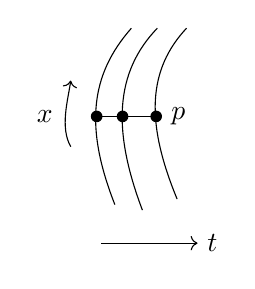
\begin{tikzpicture}[scale=0.7]
\draw (0.35,0) .. controls (-0.2,1.4) and (-0.1,2.35) .. (0.65,3.2);
\draw (0.85,-0.1) .. controls (0.3,1.35) and (0.35,2.4) .. (1.12,3.2);
\draw (1.48,0.1) .. controls (0.9,1.5) and (0.95,2.45) .. (1.65,3.2);
\draw (0.02,1.6)--(1.1,1.6);
\fill (0.02,1.6) circle (3pt);
\fill (0.49,1.6) circle (3pt);
\fill (1.1,1.6) circle (3pt);
\node[right] at (1.2,1.6) {$p$};
\draw[->] (-0.45,1.05) .. controls (-0.65,1.4) and (-0.5,1.9) .. (-0.45,2.25);
\node[left] at (-0.6,1.6) {$x$};
\draw[->] (0.1,-0.7)--(1.85,-0.7);
\node[right] at (1.85,-0.7) {$t$};
\end{tikzpicture}
\end{adjustbox}
\qquad
\nabla_t=\frac{\partial}{\partial t}+F(x,t)\frac{\partial}{\partial x}
\end{equation*}
Кас. пр-во к $\widetilde M_g$ отожд. с $\mathfrak g/\mathfrak k$.
\Unclear{GELFAND-P001258}{tangent-quotient}{В этой строке в знаменателе стоит $\mathfrak k$.}
\begin{equation*}
T(\widetilde M_g)_{(C,x,p)}
\underset{\substack{\uparrow\\\text{изоморфизм}\\\text{Кодаира—Спенсера}}}{=}
\mathbb C((x))\frac{\partial}{\partial x}\big/
\text{вект. поля, продолж. на }C\setminus\{p\}
\end{equation*}
\begin{flushright}[На полях: (всю $C$!!)]\end{flushright}

$\widetilde{\mathfrak g}$ — алг. Вирасоро.
Она действует [зачёркнуто:
\Unclear{GELFAND-P001258}{action-cancel}{в $\widetilde M_g$ [часть индекса затёрта].}]
в расслоении $d_k$.
\begin{equation*}
\begin{adjustbox}{max width=\linewidth}
\begin{tikzcd}
\widetilde M_g\arrow[d]\\M_g
\end{tikzcd}
\end{adjustbox}
\qquad
 d_k\text{ — дет. расслоение над }M_g,\text{ поднятое на }\widetilde M_g
\end{equation*}

\SourcePage{GELFAND-P001259}{unlabelled}
\underline{24.2.86.}\qquad \underline{Сем. Гельфанда}

\underline{\underline{Морозов}}\qquad
\underline{Следствия теор. Белавина—Книжника.}
\Unclear{GELFAND-P001259}{date-conflict}{В рукописном заголовке: 24.2.86.}

Явные ф-лы для бозонных струн и т.д.

Бозонная струна в крит. разм. $d=26$.

\Unclear{GELFAND-P001259}{continuation-note}{Развитие [неуверенно]} докл. Бейлинсона:
\begin{equation*}
\begin{aligned}
\sum_p\int Dx\,Dg\ \exp\int\sqrt g\,g^{ab}\partial_a x^\mu\partial_b x^\mu\,d^2\xi\prod_\alpha V_\alpha
&={}\\
&=\sum_p\int_{M_p}\frac{|d\mu_p|^2}{(\det\operatorname{Im}T)^{13}}\ K\{V\}
\end{aligned}\tag{1}
\end{equation*}
$V_\alpha$ — вершинные операторы (потом будет написано)

\noindent (2)
\SourceFigure{GELFAND-P001259}{tube-diagram}{Рисунок: трубчатая поверхность с узким левым и широким правым овальными краями, волнистыми верхней и нижней границами и маленьким отверстием посередине; у левого края видна стрелка вниз-влево. Штрихи на верхней части левого края и разрывы его контура требуют проверки по оригиналу.}

\underline{мировая пов. распр. колечка}

Взаимные превр. учитываются рассмотрением разн. топологий.

Технич. удобно счит. в нач. и в конце — точки.

\noindent (3)
\begin{equation*}
\begin{adjustbox}{max width=\linewidth}
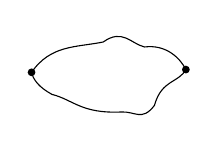
\begin{tikzpicture}[scale=0.7]
\draw (0,0.2) .. controls (0.35,0.7) and (0.8,0.65) .. (1.3,0.75)
.. controls (1.65,1.0) and (1.8,0.72) .. (2.05,0.66)
.. controls (2.45,0.71) and (2.7,0.45) .. (2.8,0.25)
.. controls (2.66,0) and (2.36,0.07) .. (2.23,-0.4)
.. controls (2.0,-0.7) and (1.88,-0.5) .. (1.62,-0.52)
.. controls (0.9,-0.55) and (0.76,-0.3) .. (0.37,-0.2)
.. controls (0.13,-0.07) and (0.03,0.07) .. (0,0.2);
\fill (0,0.2) circle (2pt);
\fill (2.8,0.25) circle (2pt);
\end{tikzpicture}
\end{adjustbox}
\end{equation*}
Тогда $V_\alpha$ — $\delta$-ф-и; переходя к пр. Фурье, получим
($\alpha$ — номер верт. опер.)
\begin{equation*}
V_\alpha(p)=\int e^{i p_\alpha x(\xi)}d^2\xi
\tag{4}
\end{equation*}
[В показателе после $p_\alpha$ зачёркнут знак:
\Unclear{GELFAND-P001259}{eq4-cancel}{возможно, $\mu$; неразборчиво.}]

Удобно брать и производные $\delta$-ф-й:
\begin{equation*}
V_\alpha(p)=\int\partial x^\mu(\xi)e^{i p_\alpha x(\xi)}d^2\xi
\tag{4'}
\end{equation*}

Для получ. прав. части в (1):

а) Интегрируем по $x$, получим
\begin{equation*}
\frac{1}{(\det\Delta_0)^{13}}\prod_\alpha\int d^2\xi_\alpha
\prod_{\alpha,\beta}\exp p_\alpha p_\beta\,G_{(reg)}(\xi_\alpha,\xi_\beta)
\tag{5}
\end{equation*}
$\Delta_0$ — лапласиан на скалярах

$G_{(reg)}$ — рег. ф-я Грина (сглаж., когда точки совпадают)

\SourcePage{GELFAND-P001260}{11}
б) Интегрируем по метрикам.
\begin{equation*}
g^{ab}=e^\varphi\delta^{ab}+(\text{бесследовые вклады})
\tag{6}
\end{equation*}
\Unclear{GELFAND-P001260}{traceless-word}{бесследовые вклады [окончание первого слова переправлено].}

Последние исключаем преоб.
\begin{equation*}
\begin{aligned}
\xi&\longrightarrow\xi+\varepsilon\\
g&\longrightarrow g+\partial G
\end{aligned}
\end{equation*}
Возникает $\det\Delta_{-1}$. Приходим к
\begin{equation*}
\int d\mu_p\,\frac{\det\Delta_{-1}}{(\det\Delta_0)^{13}}
\tag{7}
\end{equation*}
В крит. разм. исчезает зависимость от $\varphi$

Учёт нулевых мод.
\begin{equation*}
N_{\alpha\beta}^{(j)}=\langle\omega_\alpha^{(j)}\omega_\beta^{(j)}\rangle
=\int\rho^{1-j}\bar\omega_\alpha\omega_\beta\,d^2\xi
\tag{8}
\end{equation*}
Бывают $j$-дифференциалы: $f(\xi)d\xi^j$,

соотв. опр. Лапласа
\begin{equation*}
\Delta_j=\rho^{1-j}\bar\partial\rho^j\partial
\tag{9}
\end{equation*}
Нулевые моды — голом. дифференциалы.

Отсюда $\det N^{(j)}$ определён.

Получаем
\begin{equation*}
\int|d\nu_p|^2\left(\frac{\det N^{(0)}}{\det'\Delta_0}\right)^{13}
\det'\Delta_{-1}\prod d^3\xi_\alpha\prod_{\alpha,\beta}
\exp p_\alpha p_\beta\,G_{(Reg)}(\xi_\alpha,\xi_\beta)
\tag{10}
\end{equation*}
\Unclear{GELFAND-P001260}{cubic-measure}{В формуле (10) написано $d^3\xi_\alpha$.}

Здесь
\begin{equation*}
d\nu_p=\frac{dy_1\ldots dy_{3g-3}}{\det N^{(2)}}
\tag{11}
\end{equation*}
\Unclear{GELFAND-P001260}{moduli-index}{Последний индекс в числителе читается как $3g-3$.}

в правильных голом. коорд. на пр-ве модулей.
\begin{equation*}
dz\,d\bar z+f(z)dz^2+f(\bar z)d\bar z^2
\qquad\Vert\quad\text{На данной пов. }g\,dz\,d\bar z;
\tag{12}
\end{equation*}
на соседних
\begin{equation*}
\rho\,|dz+y\eta\,d\bar z|^2
\tag{13}
\end{equation*}
\noindent (14) \underline{Теор. Альфорса—Берса:}
\Unclear{GELFAND-P001260}{theorem-cancel}{[Зачёркнуто: какие-то коорд. (неуверенно); над строкой со знаком вставки: такие $y$ — (неуверенно).]}
\underline{голом. координаты} на пр-ве модулей

$y$ параметризует отклонение от пов.

\noindent (15) \underline{Утв.} (теор. Бел.—Кн.)
\begin{equation*}
\delta_y\delta_{\bar y}\frac{\det\Delta_j}{\det N^{(j)}\det N^{(1-j)}}=c_j,
\qquad c_j=6j^2-6j+1.
\tag{16}
\end{equation*}
\Unclear{GELFAND-P001260}{variation-without-log}{В (16) операторы $\delta_y\delta_{\bar y}$ стоят непосредственно перед дробью; $\log$ не написан.}
[После $c_j=$ зачёркнуто:
\Unclear{GELFAND-P001260}{final-cancel}{несколько неразборчивых математических знаков.}]

\SourcePage{GELFAND-P001261}{unlabelled}
\underline{Вопр. Гельфанда:} нет удов. теории $\det$ элл. операторов
\begin{equation*}
\det(AB)\overset{?}{=}\det A\cdot\det B
\end{equation*}
($A,B$ — элл. опер. произв. порядка, обратимые)

\SourcePage{GELFAND-P001262}{unlabelled}
\underline{3/III—86 г.}\qquad\underline{Сем. Гельфанда}

\underline{Бейлинсон}\qquad\underline{\underline{Смеш. структуры Ходжа}}
\Unclear{GELFAND-P001262}{date-conflict}{В заголовке рукописная дата: 3/III—86 г.}

\noindent (1) \underline{Опр.} \underline{Смеш. структура Ходжа} — это

1. Конечнопорожд. абелева группа $L$

и 2 фильтрации

2. $L_{\mathbb Q}:\quad\ldots\subset W_i\subset W_{i+1}\subset\ldots$

3. $L_{\mathbb C}:\quad\ldots\supset F^j\supset F^{j+1}\supset\ldots$

\underline{Условия:}
\begin{equation*}
W_a/W_{a-1}\text{ — вект. пр-во над }\mathbb Q.
\end{equation*}
На [зачёркнуто:
\Unclear{GELFAND-P001262}{crossed-word}{нём [неуверенно].}]
[вставлено над строкой: его комплексиф.]
фильтр. [зачёркнуто:
\Unclear{GELFAND-P001262}{crossed-reference}{(3) [неуверенно].}]
$(1)_3$ индуцирует фильтрацию:


No validated return is available for this job.
\SourcePage{GELFAND-P001263}{unlabelled}
\Incomplete{GELFAND-P001263}{whole-page}{No return imported; source chapter\_028/28\_part\_000011.png}
\SourcePage{GELFAND-P001264}{unlabelled}
\Incomplete{GELFAND-P001264}{whole-page}{No return imported; source chapter\_028/28\_part\_000012.png}
\SourcePage{GELFAND-P001265}{unlabelled}
\Incomplete{GELFAND-P001265}{whole-page}{No return imported; source chapter\_028/28\_part\_000013.png}
\SourcePage{GELFAND-P001266}{unlabelled}
\Incomplete{GELFAND-P001266}{whole-page}{No return imported; source chapter\_028/28\_part\_000014.png}
\SourcePage{GELFAND-P001267}{unlabelled}
\Incomplete{GELFAND-P001267}{whole-page}{No return imported; source chapter\_028/28\_part\_000015.png}
\SourcePage{GELFAND-P001268}{unlabelled}
\Incomplete{GELFAND-P001268}{whole-page}{No return imported; source chapter\_028/28\_part\_000016.png}
\SourcePage{GELFAND-P001269}{unlabelled}
\Incomplete{GELFAND-P001269}{whole-page}{No return imported; source chapter\_028/28\_part\_000017.png}
\SourcePage{GELFAND-P001270}{unlabelled}
\Incomplete{GELFAND-P001270}{whole-page}{No return imported; source chapter\_028/28\_part\_000018.png}
\SourcePage{GELFAND-P001271}{unlabelled}
\Incomplete{GELFAND-P001271}{whole-page}{No return imported; source chapter\_028/28\_part\_000019.png}
\SourcePage{GELFAND-P001272}{unlabelled}
\Incomplete{GELFAND-P001272}{whole-page}{No return imported; source chapter\_028/28\_part\_000020.png}
% GELFAND-0138. Diplomatic transcription of the ten assigned original scan frames.
% Editorial annotations are enclosed in square brackets; original images remain authoritative.
% No TeX compilation was performed.

\SourcePage{GELFAND-P001273}{20}
% Original: 2432 x 3448 px. Text occupies the upper part of the frame.
% Review crops: (265,35,1180,145) x3; (725,57,1035,121) x4;
% (140,160,1050,285) x3; (300,190,380,268) x7;
% (245,300,1510,450) x3. Coordinates: left, top, right, bottom.
коммутаторы понимаются так
\begin{equation*}
(42)\qquad x=\sum a_n z^n+\ldots\ \frac{\partial}{\partial z}
\end{equation*}
Это приводит к появл. групп в струне:
\begin{equation*}
E_8\times E_8\quad\text{или}\quad SO_{32}
\end{equation*}

\SourcePage{GELFAND-P001274}{unlabelled}
% Original: 2432 x 3448 px. Source-coordinate convention: left, top, right, bottom.
\underline{24.$\overline{\underline{\mathrm{III}}}$.86.}\qquad
\underline{Сем. Гельфанда}

\underline{\underline{Фукс.}}\qquad
\underline{Когомологии}\qquad
\underline{$\mathbb{R}^n\setminus\bigcup L_i,\quad L_i$ — плоскости}

[Над словом «плоскости» вписано: (афф.).]

$\mathbb{R}^n\supset\bigcup L_i,\quad L_i$ — афф. подпр-ва любых разм.
\begin{equation*}
X=\mathbb{R}^n\setminus\bigcup L_i.
\end{equation*}
Как считать $H_k(X)$

Пусть $L_i$ — гиперплоскости

Тогда $H_k=0$ при $k\ne0$.

Ответ (Zaslawsky, 1975)

Постр. [зачёркнуто:
\Unclear{GELFAND-P001274}{middle-cancel-01}{такое; неразборчивое слово}]
част. упор. мн-во [зачёркнуто:
\Unclear{GELFAND-P001274}{middle-cancel-02}{неразборчивые знаки}]
$A$ с элементами $\mathbb{R}^n$, $L_i$ и всевозм. их
\Unclear{GELFAND-P001274}{middle-case-endings}{непустым пересечения}

\underline{ф-я Мебиуса}
\begin{equation*}
\mu(\mathbb{R}^n)=1,\qquad\mu(L_i)=-1
\end{equation*}
\begin{equation*}
\mu(v)=-\sum_{w>v}\mu(w)
\end{equation*}
\begin{equation*}
h_0=\sum_{v\in A}|\mu(v)|\qquad\leftarrow\ \text{ф-ла Заславского.}
\end{equation*}

\underline{\underline{Пример.}}

В $\mathbb{R}^3$ коорд. плоскости
\begin{equation*}
\begin{array}{cccccccc}
\mathbb{R}^3,&L_x,&L_y,&L_z,&L_{xy},&L_{xz},&L_{yz},&0\\
1&-1&-1&-1&1&1&1&-1
\end{array}
\end{equation*}
\begin{equation*}
\sum_1^8|\pm1|=8,\quad\text{как и положено (8 октантов)}
\end{equation*}

\underline{Осн. случай}\qquad (Горецкий).

$A$ [зачёркнуто:
\Unclear{GELFAND-P001274}{lower-cancel-03}{неразборчивое слово}]
опред. так же; $A$ — част. упоряд. мн-во

\Unclear{GELFAND-P001274}{lower-dimension}{$\tau(a)$ или $r(a)$ — размерность $A$ при $a\in$ [на этом запись заканчивается]}

% Точка после заголовка: оригинал (225,2830,638,2970), независимая сверка 6x.
\underline{Теорема.}\qquad
\begin{equation*}
H_i(X)=\bigoplus_{a\in A}H_i(a),
\end{equation*}
(Горецкий-Макферсон)

где
\begin{equation*}
H_i(a)=H^{n-\tau(a)-i-1}\bigl(X_{>a},X_{(a,\mathbb{R}^n)}\bigr),
\end{equation*}
[Буква в показателе степени:
\Unclear{GELFAND-P001274}{bottom-rank-letter}{$\tau$ или $r$}.]
[Второй знак $X$ исправлен:
\Unclear{GELFAND-P001274}{bottom-overwritten-x}{$X$; прежнее начертание неразборчиво}.]

\SourcePage{GELFAND-P001275}{29}
где
% Верхняя группа: оригинал (250,0,1800,360), просмотр 3x.
\begin{equation*}
\left.
\begin{gathered}
>a\\
(a,\mathbb R^n)
\end{gathered}
\right\}
\begin{gathered}
\text{подмн-ва}\\
\text{мн-ва }A
\end{gathered}
\quad
\begin{aligned}
&\leftarrow\{b\mid b>a\}\\
&\leftarrow\{b\mid b>a\}-\{\mathbb R^n\}
\end{aligned}
\end{equation*}

$X_M$, где $M$ — част. упор. мн-во (в частн., $M\subset A$)
по опр. есть симпл. комплекс с вершинами — эл-тами $M$,
а $p$-мерн. симплексами — подмн-вами
\begin{equation*}
\{a_0<\cdots<a_p\}\subset M
\end{equation*}

(\underline{Коммент.}: по определению считается
\begin{equation*}
H^i(\varnothing,\varnothing)=
\begin{cases}
\mathbb Z,&i=-1,\\
0,&i\ne-1.
\end{cases}
\end{equation*}
Пара $(X_{>a},X_{(a,\mathbb R^n)})=(\varnothing,\varnothing)$ лишь если $a=\mathbb R^n$.

В действ., $X_{>a}$ всегда стягиваемо, так что
$H^k(X_{>a},X_{(a,\mathbb R^n)})$ сводятся к когом. $X_{(a,\mathbb R^n)}$, а именно
\begin{equation*}
H^i\left(\begin{gathered}\text{стяг.}\\\text{пр-во}\end{gathered},B\right)=
\begin{cases}
H^{i-1}(B),&i>1\\
H^0(B)/\mathbb Z,&i=1.
\end{cases}
\end{equation*}
% Начальная скобка перед «Коммент.» в оригинале далее не закрыта.

В теореме Горецкого
\textit{[зачёркнуто: \Unclear{GELFAND-P001275}{theorem-cancellation}{и; неразборчиво}]}
— Макферсона коэффициенты любые.

Частн. случай: теор. Орлика-Соломона
(\textit{[густо переписанный знак: \Unclear{GELFAND-P001275}{orlik-cancellation}{в; неразборчиво}]}
когда всё комплексное).

\underline{Пример.}

$\mathbb R^3\setminus$ коорд. плоск. и ещё одна прямая, прох. через $0$, но не
леж. ни в одной из гиперплоскостей.

$\underline{\underline{8}}$ — 0-мерных и $\underline{\underline{2}}$ 1-мерных.

% «(И.М.Г.)» написано под подчёркнутым словом «Вопрос:».
\underline{Вопрос:} (И.М.Г.) задано произв. частично упор. подмн-во; какой смысл того,
что слева (что-то вроде торического
\Unclear{GELFAND-P001275}{toric-abbreviation}{мн-зия; м-зия})

% Под заголовком в оригинале волнистая черта.
\underline{О док-ве.}

Рассм. точку
\textit{[вставлено над строкой: \Unclear{GELFAND-P001275}{proof-point-insertion}{$x_0$; $a_0$}]}
общего полож. в $\mathbb R^n$ и шар с ц. в $x_0$; будем его
раздувать, следя за изменением гомологий того, что внутри (нужн.
\Unclear{GELFAND-P001275}{proof-pronoun}{на; нам}
относит. гомологии).

% Рисунок: оригинал (1015,3120,1255,3310), просмотр 6x.
% Видимые контуры, две близкие косые черты и штриховка; надписей в рисунке нет.
\begin{center}
\begin{adjustbox}{max width=\linewidth}
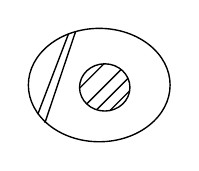
\begin{tikzpicture}[line width=0.5pt]
\draw (0,0) ellipse (0.9 and 0.72);
\draw (0.07,-0.03) ellipse (0.32 and 0.3);
\draw (-0.78,-0.37)--(-0.39,0.65);
\draw (-0.69,-0.48)--(-0.3,0.68);
\clip (0.07,-0.03) ellipse (0.32 and 0.3);
\draw (-0.45,-0.24)--(0.15,0.36);
\draw (-0.29,-0.37)--(0.32,0.24);
\draw (-0.1,-0.38)--(0.48,0.2);
\draw (0.07,-0.39)--(0.6,0.14);
\end{tikzpicture}
\end{adjustbox}
\quad
\parbox{7cm}{шар с выколотой прямой\\
$\operatorname{mod}$ выкинут. меньшего шара.}
\end{center}

\SourcePage{GELFAND-P001276}{unlabelled}
На самом деле к вычисл. отн. гом. дело не сводится.

\textit{[зачёркнуто:
\Unclear{GELFAND-P001276}{top-cancelled-inclusion}{$D_{\text{мал}}\subset D_{\text{бол}}$; $D_{\text{мал}}\supset D_{\text{бол}}$}]}
$D_{\text{мал}}\subset D_{\text{бол}}$

\begin{equation*}
H_*(D_{\text{бол}})=H_*(D_{\text{мал}})\oplus H_*(D_{\text{бол}},D_{\text{мал}})
\end{equation*}

если точная послед. расщепляется, но это здесь проверяется
чисто геом. образом.

(1) \textit{[зачёркнуто: Когда]} \underline{Пример}, когда довод. до конца.
\begin{equation*}
\begin{aligned}
\operatorname{Codim}L_i&=k\qquad\text{(не зав. от }i\text{)}\\
\operatorname{codim}(L_{i_1}\cap\cdots\cap L_{i_q})&\quad\text{делится на }k
\end{aligned}
\end{equation*}
($k=1$ выполнено и в компл. сит. выполнено)

Но даже \textit{[зачёркнуто: \Unclear{GELFAND-P001276}{real-example-cancellation}{при; неразборчиво}]}
в $\mathbb R^4$ при $k=2$ это не обязательно комплексная
ситуация!! (Пример Горецки есть)

\underline{Вопрос} (ИМГ): при каких усл. сущ. компл. структ., в к-рой
все они станут комплексными?

% Под следующими двумя заголовками в оригинале волнистое/прерывистое подчёркивание.
\underline{Пример Горецки.}

\underline{Теор. Паппа.}

% Рисунок: оригинал (775,1620,1195,1870), просмотр 5x.
% Два ряда по три обведённые точки, шесть соединяющих отрезков,
% три отмеченные внутренние точки и проходящий через них пунктир. Надписей нет.
\begin{center}
\begin{adjustbox}{max width=\linewidth}
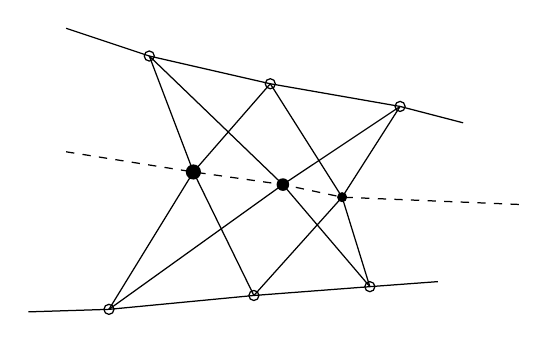
\begin{tikzpicture}[x=0.016cm,y=-0.016cm,line width=0.45pt]
\coordinate (p276a) at (106,32);
\coordinate (p276b) at (202,54);
\coordinate (p276c) at (305,72);
\coordinate (p276d) at (74,233);
\coordinate (p276e) at (189,222);
\coordinate (p276f) at (281,215);
\coordinate (p276p) at (141,124);
\coordinate (p276q) at (212,134);
\coordinate (p276r) at (259,144);
\draw (40,10)--(p276a)--(p276b)--(p276c)--(355,85);
\draw (10,235)--(p276d)--(p276e)--(p276f)--(335,211);
\draw (p276a)--(p276p)--(p276e);
\draw (p276a)--(p276q)--(p276f);
\draw (p276b)--(p276p)--(p276d);
\draw (p276b)--(p276r)--(p276f);
\draw (p276c)--(p276q)--(p276d);
\draw (p276c)--(p276r)--(p276e);
\draw[dashed] (40,108)--(p276p)--(p276q)--(p276r)--(405,150);
\draw (p276a) circle (4);
\draw (p276b) circle (4);
\draw (p276c) circle (4);
\draw (p276d) circle (4);
\draw (p276e) circle (4);
\draw (p276f) circle (4);
\fill (p276p) circle (6);
\fill (p276q) circle (5);
\fill (p276r) circle (4);
\end{tikzpicture}
\end{adjustbox}
\end{center}

При компл. шевелении ситуация сохраняется, а при вещ. нет!!

Пусть вып. условия (1). Тогда
\begin{equation*}
\forall a,\ H_i(a)\ne0\quad\text{только для одного }i:
\end{equation*}
% Вопросительный знак над равенством и штрих при m принадлежат оригиналу;
% область (570,2235,1060,2400) просмотрена при увеличении 8x.
\begin{equation*}
i\overset{?}{=}m'(k-1)
\end{equation*}
\begin{equation*}
H_i(a)=\underbrace{\mathbb Z\oplus\cdots\oplus\mathbb Z}_{|\mu(a)|}
\end{equation*}

% Под словами «Вопрос И.М.Г.» волнистая черта.
\underline{Вопрос И.М.Г.} Как найти правильный базис когомологий?

\SourcePage{GELFAND-P001277}{30}
% Original source: 2432 x 3448 pixels. Cancellations and insertions are documentary annotations.
[Зачеркнуто: \Unclear{GELFAND-P001277}{top-cancel}{неразборчиво}.]

\underline{\underline{Варченко.}}\quad
\underline{Смешанные структуры Ходжа}

Это 2 фильтрации в лин. пр-ве: возраст. и убывающая

(в когом. компл. мн-ия)\qquad ходжева и весовая

[Под «весовая» проведён короткий штрих к приписке:]
тополог. (не мен. при деф. компл. структуры)

Они прав. согласованы и прав. меняются при изм. мн-ия.
Будет пример этого.

\underline{Когомологии проект. неособого мн-ия (компактного)}

В когом. есть \underline{чистая структ. Ходжа}
\begin{equation*}
0\subset F^k\subset\cdots\subset F^1\subset F^0=H^k\tag{1}
\end{equation*}
\Unclear{GELFAND-P001277}{filtration-index}{Показатель перед $F^0$: $F^1$ или $F^{-1}$; верхняя черта слита с буквой $F$.}
Здесь
\begin{equation*}
\begin{aligned}
F^s=\bigl\{[\omega],\quad&\omega\text{ — замкн. комплекснозн. дифф. форма,}\\
&\omega=\sum a_i\,dz_{i_1}\wedge\cdots\wedge dz_{i_s}\wedge\cdots\bigr\}
\end{aligned}\tag{2}
\end{equation*}
[Под $dz_{i_1}\wedge\cdots\wedge dz_{i_s}$ и под последующим многоточием
проведены две отдельные нижние скобки; ниже между ними: «всего $k$».]

[Под формулой:] $\exists$ предст.:
($\ge s$ голом. дифф. в лок. записи)

Измен. компл. структ. $\Rightarrow$ подпр. непр. меняются.

\underline{Пример весовой фильтрации.}

В $\mathbb C\setminus\{0\}$ отождествим 2 точки $*,*$

Топологически:
\begin{center}
\begin{adjustbox}{max width=\linewidth}
\begin{tikzpicture}[x=1cm,y=1cm]
\draw (0,1.5) ellipse (0.4 and 0.2);
\draw (-0.4,1.5) -- (-0.48,0.2);
\draw (0.4,1.5) -- (0.32,0.2);
\draw (-0.48,0.2) arc (180:360:0.4 and 0.2);
\draw[dashed] (-0.48,0.2) arc (180:0:0.4 and 0.2);
\draw (-0.22,0.85) circle (0.04);
\draw (0.13,0.87) circle (0.04);
\node[anchor=west] at (0.9,0.9) {цил. с отожд. 2-мя точками.};
\end{tikzpicture}
\end{adjustbox}
\end{center}
\begin{equation*}
\dim H^1(X)=2
\end{equation*}
\SourceFigure{GELFAND-P001277}{cylinder-cycles}{Справа ниже первого цилиндра нарисован второй цилиндр. От слов «цил. с отожд. 2-мя точками» к его верхнему овалу спускается штрих. В середине цилиндра овальный контур с подписью $a$ и стрелкой вправо на передней дуге; ниже видны знак $\times$ слева, звёздочка справа выше и соединяющая их кривая. Справа подпись «2 цикла.» и два указателя влево: прямой к среднему овалу и изогнутый к нижней кривой. Точная геометрия нижнего соединения остаётся неуверенной.}

В $H_1$ [верхний индекс зачеркнут:
\Unclear{GELFAND-P001277}{homology-index-cancel}{возможно, $1$; неуверенно}]
имеется 1-мерн. подпр-во, порожд. циклом $a$

$W$ [зачеркнуто: \Unclear{GELFAND-P001277}{weight-space-cancel}{неразборчиво}]
$\subset H^1(X)$

[Под зачёркиванием, с косым указателем:] аннулятор этого 1-мерного подпр-ва.

[Под $W$, с вертикальным штрихом:] весовое. пр-во.

\underline{Другой способ появл. смеш. структур Ходжа, связ. с асимптотиками.}

Рассм. вещ.-анал. ф-ю
$f:\mathbb R^n\underset{\text{аналит.}}{\longrightarrow}\mathbb R.$

$\omega=h\,dx_1\wedge\cdots\wedge dx_n$ с комп. $\mathrm{supp}$
\begin{equation*}
\omega\mapsto\int_{\mathbb R^n}f^\lambda\omega\tag{3}
\end{equation*}
продолж. [зачеркнуто:
\Unclear{GELFAND-P001277}{continuation-cancel}{«на» или «не»; неуверенно}]
на всю $\mathbb C$ с полюсами в точках
\begin{equation*}
\int_{\mathbb R^n}f^\lambda\omega
=\sum a_{k,\alpha}(\omega)\frac{1}{(\lambda+\alpha)^k}\tag{4}
\end{equation*}
[Справа от (4) зачеркнут знак:
\Unclear{GELFAND-P001277}{bottom-symbol-cancel}{$\alpha$ или $a$; неуверенно}.]

\SourcePage{GELFAND-P001278}{unlabelled}
% Original source: 2432 x 3448 pixels. The source has no confidently visible page label.
$k$ — проявл. весовой [зачеркнуто: стр. Ходжа] фильтрации

$\alpha$ — 〃 — ходжевой — 〃 —

2 параметра: целый $k$ и рацион. $\alpha$
всегда явл. точным проявл. смеш. стр. Ходжа.

\underline{Компл. случай.}

$f:(\mathbb C^n,0)\longrightarrow(\mathbb C,0),\quad f$ голом.

$0$ — изолир. крит. точка

Рассм. слой $f^{-1}(0)$ — особая с изолир. особ. точкой $0$.

Рассм. в $\mathbb C^n$ мал. шар и в $\mathbb C$ мал. диск (много меньше) $\Rightarrow$

$\Rightarrow$ получ. голом. слои (вовсе не алгебраические)

\SourceFigure{GELFAND-P001278}{milnor-fibration}{Слева круглый контур с несколькими почти вертикальными линиями; две центральные линии имеют обращённые друг к другу изгибы. Справа вверху подпись $\mathbb C^n$. Из круга вниз направлена стрелка с подписью $f$ к наклонному четырёхугольнику. Внутри четырёхугольника овал; слева от овала знак, похожий на $D$ или «Д», справа от четырёхугольника $\mathbb C$. Точные соединения центральных линий и чтение внутренней подписи не установлены.}

$X_t=f^{-1}(t)$ [зачеркнуто:
\Unclear{GELFAND-P001278}{fiber-cancel}{возможно, «в \ldots»; остальное неразборчиво}]
— один слой.

$(n-1)$-мерн. компл. мн-ие.

\underline{Теор. Милнора:}
\begin{equation*}
X_t\underset{\text{гом. экв.}}{\sim}
\underbrace{S^{n-1}\vee\cdots\vee S^{n-1}}_{\mu\text{ — число Милнора крит. точки}}
\end{equation*}

$\underline{n=2}\ \Rightarrow\ X_t$ — некомп. компл. кривая, связная

На границе [зачеркнуто:
\Unclear{GELFAND-P001278}{boundary-cancel}{возможно, «слоя»; неуверенно}]
что-то отрезается

\SourceFigure{GELFAND-P001278}{punctured-surface}{Слева у формулы (5) изображён вытянутый замкнутый округлый контур, сужающийся кверху, с небольшим верхним овалом и узким замкнутым контуром внутри. У верхнего овала короткие боковые штрихи. Подписи и стрелки отсутствуют. Пространственная интерпретация этих контуров не уточняется.}
\begin{equation*}
\mu=2g-(\text{число дырок})+1\tag{5}
\end{equation*}
\Unclear{GELFAND-P001278}{milnor-hole-signs}{Математический смысл «число дырок» в (5) не установлен: возможная описка или иная конвенция. Видимые знаки в $2g-(\text{число дырок})+1$ сохранены.}

\begin{adjustbox}{max width=\linewidth}
\begin{tikzpicture}[x=1cm,y=1cm]
\draw (0,0) .. controls (-0.24,0.34) and (-0.2,0.8) .. (0.03,0.85)
 .. controls (0.48,0.98) and (0.32,0.4) .. (0,0)
 .. controls (-0.5,-0.5) and (-0.14,-1.0) .. (0.26,-0.72)
 .. controls (0.58,-0.45) and (0.22,-0.18) .. (0,0);
\fill (0,0) circle (0.035);
\node[anchor=west] at (0.9,0) {Получ. букет окружностей.};
\end{tikzpicture}
\end{adjustbox}

При обходе возникает тр. монодромии
$M:H^{n-1}(X_t)\longrightarrow H^{n-1}(X_t)$

[Зачеркнуто: \Unclear{GELFAND-P001278}{cancelled-heading}{возможно, «Интегралы»; неуверенно}.]

\underline{Вопр. Гельфанда:} что для
$\int f_1^{\lambda_1}f_2^{\lambda_2}\cdots f_k^{\lambda_k}$ — ?

Для $\mathbb C^n\to\mathbb C^k$ будет ли [зачеркнуто:
\Unclear{GELFAND-P001278}{several-functions-cancel}{неразборчиво}]
возникать что-то вроде смеш. стр. Ходжа?

\underline{Вопр. И.М.Г.:} что [зачеркнуто:
\Unclear{GELFAND-P001278}{quadratic-pair-cancel}{неразборчиво}]
возник. при отобр., зад. парой кв. форм?

Рассмотрим форму

$\omega=h\,dz_1\wedge\cdots\wedge dz_n,\qquad h$ — голом.

На неособом слое можно рассм.

$\omega/df$ — голом. $(n-1)$-форму

Рассм. выделенный цикл в слое и распростр. его на соседние слои
по непр. — получим многозн. сем-во циклов $\delta(t)$
\Unclear{GELFAND-P001278}{last-mark}{После $\delta(t)$ короткий восходящий штрих: запятая или завершающий росчерк.}

\SourcePage{GELFAND-P001279}{31}
% Original source: 2432 x 3448 pixels.
\begin{equation*}
I(t)=\int_{\delta(t)}\frac{\omega}{df}\tag{6}
\end{equation*}

Прох. через крит. знач. — теор. Морса

обход вокруг $0$ — теор. Пикара--Лефшеца

Эти 2 аспекта дают 2 фильтрации.

\underline{Весовая фильтрация}
[над окончанием «Весовая»:
\Unclear{GELFAND-P001279}{weight-ending-mark}{зачёркнутая или исправленная буква, возможно «й»}]
— фильтрация [зачеркнуто:
\Unclear{GELFAND-P001279}{operator-word-cancel}{неразборчиво}]
лин. оператора $M$ по его жорд. клеткам.

Надо у $M$ изготовить нильпотентную часть и её фильтрацию

\SourceFigure{GELFAND-P001279}{jordan-filtration}{Слева девять прямоугольных клеток: в первых двух горизонтальных рядах по три, в третьем две, в нижнем одна. В каждом из первых двух рядов две соединяющие стрелки направлены вправо; в третьем ряду одна стрелка вправо. Между столбцами и снаружи проходят вложенные линии, сначала почти вертикальные, затем поворачивающие вправо; на некоторых нижних участках видны короткие утолщённые штрихи. Справа длинная почти вертикальная линия с маленькими петлями у концов. Правее надписи: «(рисуем клетки)», «симметрично отн. нек-рой оси.», ниже указатель влево и подчёркнутое «фильтрация.». Точная геометрия вложенных линий и значение мелких штрихов не реконструированы.}

1) Соб. вект. в самых больших жорд. клетках

2) Присоед. соб. вект. в меньших кл. [зачеркнуто:
\Unclear{GELFAND-P001279}{second-step-cancel}{неразборчиво}]

и т.д.

Разные соб. знач. компонуются в зав. от того $\lambda=1$ или $\lambda\ne1$

[Под $\lambda=1$, с указателем:] средний вес $n$

[Под $\lambda\ne1$:] вес $n-1$ всем

\begin{equation*}
I(t)=\int_{\delta(t)}\frac{\omega}{df}
=\sum a_{k,\alpha}\,t^\alpha(\ln t)^k\tag{7}
\end{equation*}

[Зачеркнуто: \Unclear{GELFAND-P001279}{coefficient-word-cancel}{возможно, «где»; неуверенно}]
$a_{k,\alpha}$ линейно зависят от $\omega$ и от $\delta$

$e^{2\pi i\alpha}=$ соб. числа $M$

$k=$ [вставлено над строкой: размер] жорд. клеток опер. $M$

\underline{Ссылки:}

1) Варченко, ДАН, 1980

2) [зачеркнуто: \Unclear{GELFAND-P001279}{reference-cancel}{неразборчивый знак}]
конструкция в ВИНИТИ

3) Книга по особенностям

\SourcePage{GELFAND-P001280}{unlabelled}
% Original: 2432 x 3448 px. All writing lies above y=1100.
% Review crops: (330,180,1780,345) x3; (1135,260,1215,335) x9;
% (275,378,1540,602) x3; (325,600,2240,840) x3;
% (270,945,1840,1075) x3; (850,960,1100,1065) x6.
\underline{Главный член асимптотики.}

\begin{equation*}
(8)\qquad
I(t)=t^{\alpha(\omega)}
\left(\sum a_{k,0}^{\omega}+a_{k,1}^{\omega}\ln t+\ldots\right)
+o\left(t^{\alpha(\omega)}\right)
\end{equation*}

Смеш. структ. Ходжа получ. из 1-го члена.

Многочл. Бернштейна — из всех членов.

\begin{equation*}
V_\alpha=
\{\text{классы главн. частей форм }\omega,\ \alpha(\omega)=\alpha\}
\quad\text{— классы когомологий}
\end{equation*}

($\alpha$ — рац.)
\begin{equation*}
V_\alpha\subset V_{\alpha+1}
\end{equation*}

Варченко интересовался полунепр. главн. частей асимптотики.

\SourcePage{GELFAND-P001281}{unlabelled}
% Original frame 2432 x 3448. Reading order top to bottom.
% Source date was inspected at 5x, bbox (213,60,598,171): visible year 86.
7/$\overline{\underline{\mathrm{IV}}}$—86 г. \quad \underline{Сем. Гельфанда.}

\underline{\underline{Чередник.}} \quad \underline{Янгиан.}

Определение янгиана.

\begin{equation*}
\underset{\text{матр. }N\times N}{M_N}\supset\{\mathbf{1}^{k\ell}\},
\qquad \mathbf{1}\text{ — матр. ед-иница}
\end{equation*}
[От $\{\mathbf{1}^{k\ell}\}$ проведена косая черта к надписи: станд. базис.]
(1 на месте $k,\ell$, остальные $0$)
\begin{equation*}
(\mathbf{1}^{k\ell})_{ij}=\delta_{ik}\delta_{j\ell}.
\end{equation*}

\begin{equation*}
\det(\mathbf{1}+\lambda^{-1}\Unclear{GELFAND-P001281}{matrix-letter}{V\text{ / }U})\text{ — ?}
\end{equation*}
\begin{equation*}
\Unclear{GELFAND-P001281}{matrix-letter}{V\text{ / }U}=\sum_{k,\ell=1}^{N}\mathbf{1}^{k\ell}e_{\ell k}
\in M_N\bigl(U(g\ell_N)\bigr)
\end{equation*}
\begin{equation*}
\{e_{\ell k}\}\subset U(g\ell_N)
\end{equation*}

% Cancelled formula at original bbox (334,919,609,1098), examined at 7x.
(1) [Зачёркнуто: \Unclear{GELFAND-P001281}{eq1-cancelled}{${L_n(\lambda)}$ / ${U_n(\lambda)}$}.]
\begin{equation*}
L_n(\lambda)=E\mathbf{1}
+\sum_{k,\ell}\sum_{q=1}^{n}\frac{1}{\lambda^q}
\mathbf{1}^{k\ell}E_{\ell k}^{q-1}=
\end{equation*}
коэфф. — буквы $E_{\ell k}^{q}$ (с 3-мя индексами)
\begin{equation*}
=\begin{pmatrix}
E&&&0\\
&E&&\\
&&\ddots&\\
0&&&E
\end{pmatrix}+\cdots
\end{equation*}
[Справа:] (индекс $n$ дальше иногда опускается)

Положим
\begin{equation*}
R(\lambda):=\mathbf{1}\otimes\mathbf{1}
+\frac{1}{\lambda}\sum\mathbf{1}^{k\ell}\otimes\mathbf{1}^{\ell k}
\in M_N^{\otimes2}=M_{N^2}
\tag{2}
\end{equation*}
(обычная матричная ф-я).

Рассм. ур-е:
\begin{equation*}
R(\lambda_1-\lambda_2)
\Unclear{GELFAND-P001281}{eq3-ink-mark}{\text{точка / зачёркнутый знак}}
{}^{1}L_n(\lambda_1)\,{}^{2}L_n(\lambda_2)
={}^{2}L_n(\lambda_2)\,{}^{1}L_n(\lambda_1)R(\lambda_1-\lambda_2),
\tag{3}
\end{equation*}
\begin{equation*}
{}^{1}L_n=L_n\otimes\mathbf{1},\qquad
{}^{2}L_n=\mathbf{1}\otimes L_n
\end{equation*}
В коэфф. квадратично входят буквы $E_{\ell k}^{q}$

Требуется, чтобы (3) вып. тождественно по $\lambda_1,\lambda_2$.

Ур-е (3) наз. ур-ями YBF (Янга–Бакстера–Фадде\Unclear{GELFAND-P001281}{ybf-name-correction}{е / нечитаемая исправленная буква}ва).
Оно равносильно алг. системе (4)–(5):
\begin{equation*}
[E,E_{k\ell}^{q}]=0
\tag{4}
\end{equation*}
\begin{equation*}
\begin{aligned}
[E_{ij}^{p},E_{k\ell}^{q}]={}&
\delta_{jk}EE_{i\ell}^{p+q}-\delta_{\ell i}EE_{kj}^{p+q}\\
&+\sum_{a+b=p+q-1}^{a<p\leq b}
\bigl(E_{kj}^{a}E_{i\ell}^{b}-E_{kj}^{b}E_{i\ell}^{a}\bigr)
\end{aligned}
\tag{5}
\end{equation*}

(6) По определению $E_{k\ell}^{n+i}=0$ при $i\geq0$

\SourcePage{GELFAND-P001282}{43}
% Original frame 2432 x 3448. Source leaf label 43 at upper right.
(7) \underline{Утв.} При $E=1$ и если отбросить последний член в (5), то
получится
\begin{equation*}
U\bigl(g\ell_N[t]/(t^n)\bigr).
\end{equation*}
[Внутри $U(\cdots)$, перед $g\ell_N$, зачёркнуто:
\Unclear{GELFAND-P001282}{eq7-cancelled}{${g}$ / нечитаемый знак}.]
(оберт. алгебра)

\underline{Определение Янгиана.}
\begin{equation*}
Y^n=\mathbb{C}_{\text{\Unclear{GELFAND-P001282}{eq8-abbreviation}{некоммут / некомму}}}
[E_{ij}^{q};E]\,/(4)\text{–}(5)
\tag{8}
\end{equation*}

[! в кружке] ИМГ: \underline{Идея:} перест. соотношения не как в алг. Ли,
а $x_1x_2-x_2x_1$ — полином степ 2!
Опис. квадр. алгебр — правильный мат. вопрос.
(Интересно, когда вып. теорема-Пуанкаре–биркгоф–витта).

Ч. $R$-матрицу (2) можно брать также любой
[Вставлено над строкой: рациональной,]
тригонометрической и эллиптической (с соотн. согласованности)

[! в кружке] \underline{Задача} (ИМГ) Расклассифицировать, чтобы $n$-й степ. было нужное число штук.

Ассоциативность тоже не обязательна

(Jackiw: ассоциат. — коцикл 3-й степ.)

Ч.

(9) \underline{\underline{Утв.}} При $E=1$ будет $Y^1=U(g\ell_N)$

(универс. оберт. алгебра)

(10) \underline{Теор. Замолодчикова} При рациональном $R$ теор. П.-Б.-В. выполн.
тогда и только тогда, когда вып. соотн. $R\ R\ R=R\ R\ R$

\underline{\underline{Коган}} \underline{\underline{Ян}} \qquad
\underline{Струны и калибровочные поля.}

\begin{equation*}
\underline{\text{Калибровочная симметрия}}
\overset{?}{\longleftarrow}\text{ струна}
\end{equation*}

% Scattering sketch and labels, source bbox (92,2320,2212,2790), checked at 3x.
\begin{center}
\begin{adjustbox}{max width=\linewidth}
\begin{tikzpicture}[x=1cm,y=1cm]
\node at (-1.4,0) {(1)};
\node at (0,1.65) {$S$-матрица};
\draw (0,0) circle (0.43);
\draw (-0.32,0.35) -- (-0.95,1.05);
\draw (0.31,0.37) -- (0.79,1.1);
\draw (-0.98,0.02) -- (-0.51,0.02);
\draw (-0.34,-0.33) -- (-1.0,-0.92);
\draw (0.31,-0.35) -- (0.64,-0.99);
\node at (-1.0,1.22) {$\lambda_1\ p_1$};
\node at (0.8,1.27) {$\lambda_2\ p_2$};
\draw[->] (1.55,0.02) .. controls (1.73,0.25) and (1.82,-0.1) .. (2.04,0.03)
.. controls (2.2,0.14) and (2.35,-0.11) .. (2.5,-0.05) -- (3.1,-0.05);
\node at (5.55,0) {$A(p_1,\lambda_1;p_2,\lambda_2;\ldots)$};
\node at (5.55,-0.72) {(амплитуды рассеяния)};
\node at (5.55,1.7) {$\lambda_j$ — кв. числа, $p_j$ — импульсы};
\node at (5.55,1.27) {(напр. момент, цвет и т. п.)};
\node at (5.35,0.85) {всё, что не импульс.};
\draw[->] (8.2,0.2) -- (9.15,0.85);
\node at (9.9,1.02) {теория поля};
\end{tikzpicture}
\end{adjustbox}
\end{center}

\SourceFigure{GELFAND-P001282}{angular-momentum-graph}{Оси $J$ (угловой момент) и $m^2$; пять восходящих почти параллельных прямых. Три кружкообразные отметки на вертикальной оси и три справа, одна над другой; нижняя правая отметка лежит на горизонтальной оси. Возле неё обозначен угол $\alpha'$. Различие пустых и закрашенных отметок неясно. Подпись под горизонтальной осью: $(m\text{ — масса})$.}

Угл. момент всегда квантуется.

($\alpha'$ — угол —
— натяж. струны)

[Зачёркнуто: \Unclear{GELFAND-P001282}{bottom-cancelled}{Угл. / нечитаемое слово}.]
Предел $\alpha'\to0$ $\Rightarrow$ Ян–Миллс или Эйнштейн


\SourcePage{GELFAND-P001283}{unlabelled}
Действие для струны:
\begin{equation*}
S=\frac{1}{2\pi\alpha'}\int g^{ab}\sqrt g\,\partial_a x^\mu\partial_b x^\mu\,d^2\xi
\tag{2}
\end{equation*}
При переходе к
\begin{equation*}
S=\frac{1}{2\pi\alpha'}\int\partial_a x^\mu\partial_a x^\mu\,d^2\xi
\tag{3}
\end{equation*}
возникает проблема духов: не тот знак при $x^0$.

[Между строками перед (4) вписано: Разложим по осцилляторам]
\begin{equation*}
x^\mu(\sigma,\tau)=x^\mu+p^\mu\tau
+i\sum_{n=1}^\infty
\left(\frac{a_n}{\sqrt n}e^{in\tau}\cos n\sigma
+\frac{a_{-n}}{\sqrt n}e^{-in\tau}\cos n\sigma\right)
\tag{4}
\end{equation*}
\Unclear{GELFAND-P001283}{oscillator-normalization}{[В (4) оба знаменателя прочитаны как $\sqrt n$.]}

($\tau$ — время)

$\sigma$ — параметр вдоль струны

[Справа рисунок:]
\begin{center}
\begin{adjustbox}{max width=\linewidth}
\begin{tikzpicture}[x=1cm,y=-1cm]
\draw (0,2.06) .. controls (.55,1.3) and (.85,1.0) .. (1.10,.86)
 .. controls (1.55,.5) and (1.72,.2) .. (2.24,0);
\draw (1.79,2.96) .. controls (2.10,2.51) and (2.30,2.22) .. (2.49,2.01)
 .. controls (2.86,1.62) and (4.19,1.47) .. (4.29,.96);
\draw[->] (1.10,.86) .. controls (1.48,.82) and (1.77,.97) .. (1.98,1.31);
\draw (1.98,1.31) .. controls (2.02,1.35) and (2.08,1.40) .. (2.139,1.493)
 .. controls (2.26,1.75) and (2.36,1.93) .. (2.49,2.01);
\node at (2.17,1.17) {$\sigma$};
\draw[->] (2.139,1.493) .. controls (2.51,1.06) and (3.05,.72) .. (3.74,.55);
\node at (3.80,.24) {$\tau$};
\end{tikzpicture}
\end{adjustbox}
\end{center}

Оператор Вирасоро:
\begin{equation*}
L_n=:\sum_m a_n a_{m-n}:
\tag{5}
\end{equation*}
\Unclear{GELFAND-P001283}{virasoro-indices}{[В (5) прочитано $a_n a_{m-n}$.]}

$a_k$ при $k>0$ — опер. уничтожения

$a_k$ при $k<0$ — —"— рождения

(6) \underline{Состояния:}
\begin{equation*}
\begin{aligned}
\underset{\text{(вакуум)}}{|0\rangle}&\mapsto\text{тахион}\\
a_{-1}^\mu|0\rangle&\quad\text{— безмасс вект. частица}\\
a_{-1}^\mu a_{-1}^\nu|0\rangle,&\qquad a_{-2}^\mu|0\rangle\qquad\text{и т.д.}
\end{aligned}
\end{equation*}
Вообще: легко проверить, что
\begin{equation*}
M^2=-1+\sum_{n=1}^\infty:a_{-n}^\mu a_n^\mu:
\tag{7}
\end{equation*}
Среди состояний (6) много лишних: например,
\Unclear{GELFAND-P001283}{negative-norm-state}{$|a_{-1}^0|0\rangle$ [нижний индекс исправлен]}
имеет неправильную норму

[Между строками вписано: В классике есть]

Усл. репараметризационной инвариантности
\begin{equation*}
\left(p^\mu(\sigma)\pm\frac{\partial x^\mu(\sigma)}{\partial\sigma}\right)^2=0.
\tag{8}
\end{equation*}

\SourcePage{GELFAND-P001284}{44}
Из (8) следует
\begin{equation*}
\sum_n L_n e^{in\sigma}=0\quad\Rightarrow L_n=0
\tag{9}
\end{equation*}
[Под первым $L_n$, с выносной чертой: это коэфф. разл. в (8).]

Но в квант. теории это невозможно, т.к. есть центральный заряд:
\begin{equation*}
[L_n,L_m]=(n-m)L_{n-m}+\frac D{12}(n^3-n)\delta_{n+m,0}
\tag{10}
\end{equation*}
\Unclear{GELFAND-P001284}{virasoro-bracket-index}{[В (10) прочитано $L_{n-m}$.]}

[Между строками вписано: заметим, что]
\begin{equation*}
[a_n^\mu,a_m^\nu]=n\delta_{n+m,0}\eta^{\mu\nu}
\tag{11}
\end{equation*}
Условие на состояние
\begin{equation*}
L_n|\Psi\rangle=0\qquad\text{при всех }n.
\tag{12}
\end{equation*}
потребовать нельзя.

Наложим условия:
\begin{equation*}
L_n|\Psi\rangle=0,\quad n\ge1,\quad(L_0-1)|\Psi\rangle=0
\tag{13}
\end{equation*}
\Unclear{GELFAND-P001284}{classical-initial}{Классич. [начальная буква обведена или исправлена]}
условия (9) надо трактовать через средние:
\begin{equation*}
\langle\Psi|L_n|\Psi\rangle=0,
\tag{14}
\end{equation*}
что вытекает из (13) при любом $n\ne0$.

(15) \underline{Теор. струны} — квантовая мех. большого гильб. пр-ва,
в \Unclear{GELFAND-P001284}{theory-correction}{к-ром [исправлено]}
наложены усл. (13).

Это старая теория струн.

Теперь \underline{струнная теория поля}.

(Впервые 71–72 г.)

2 способа
\begin{equation*}
\begin{aligned}
\text{Рассм.}\quad |0\rangle&\rightsquigarrow\varphi(x)\\
a_{-1}^\mu|0\rangle&\rightsquigarrow A^\mu(x)
\end{aligned}
\end{equation*}
[У $A^\mu(x)$ зачёркнут нижний индекс:
\Unclear{GELFAND-P001284}{vector-field-correction}{$\mu$?}.]
\begin{equation*}
a_{-1}^\mu a_{-1}^\nu|0\rangle;\quad a_{-2}^\mu|0\rangle
\rightsquigarrow h^{\mu\nu}(x), B^\mu(x)
\end{equation*}
Более популярно: рассмотрим

\SourcePage{GELFAND-P001285}{unlabelled}
\begin{equation*}
\left(\varphi(x)+A_\mu(x)a_{-1}^\mu
+h_{\mu\nu}(x)a_{-1}^\mu a_{-1}^\nu
+B_\mu(x)a_{-2}^\mu+\ldots\right)|0\rangle
\tag{16}
\end{equation*}
В старой записи через $x^\mu(\sigma)\mapsto x^\mu,a_n^\mu$

это был ф-л от контура.

(16) — состояние (набор состояний),

точке $x(\sigma)\rightsquigarrow$ состояние $\Phi(x(\sigma))$. (поле на струне)

Аналог. разл. можно получить
\begin{equation*}
\Phi[x(\sigma)]=\Phi[x,a_n^\mu]
\end{equation*}
(17) \underline{Прав. перехода}

Разложим в ряд Тейлора по $a_n^\mu$,

коэфф. при $a_n^\mu$ с $n>0$ несущественны (нефизичны),

их надо выкинуть и оставить только операторы \underline{рождения}.

[Перед (18) зачёркнуто:
\Unclear{GELFAND-P001285}{cancelled-before18}{Из?}.]

(18) Репараметриз. инвариантность будет при условиях (13).

$\Rightarrow$ поля не независимы.

[Между строками вписано: Вычисляя по ф-ле (5), получим]
\begin{equation*}
L_1=a_1^\mu\frac{\partial}{\partial x^\mu}+\ldots
\tag{19}
\end{equation*}
Применяя к (16), получаем:
\begin{equation*}
\partial_\mu A_\mu(x)=0,
\tag{20}
\end{equation*}
\begin{equation*}
\partial_\mu h_{\mu\nu}=A_\nu.
\tag{21}
\end{equation*}
\Unclear{GELFAND-P001285}{tensor-vector-relation}{[В правой части (21) прочитано $A_\nu$.]}

(с точн. до коэффициентов)

Получ. усл. калибровки Лоренца (20).

Итак, вместо наложения связей рассмотрим
\begin{equation*}
\delta|\Psi\rangle=\sum_{n=1}^\infty b_n L_{-n}|\Phi\rangle,
\tag{22}
\end{equation*}
[Под $\delta$, с выносной чертой: вариация состояния]

$b_n$ — произв. параметры.

Будем действ., чтобы поддерживать эту инвариантность.
\begin{equation*}
\delta A_\mu=\partial_\mu\varepsilon+[\varepsilon,A]
\tag{23}
\end{equation*}

\SourcePage{GELFAND-P001286}{45}

\begin{equation*}
\begin{aligned}
(\delta\varphi(x)+\delta A_\mu(x)a_\mu^{-1}\ldots)\lvert0\rangle
&=b_1\frac{\partial}{\partial x^\mu}a_\mu^{-1}
(\varepsilon(x)+a_\mu^{-1}b_\mu(x)+\ldots\lvert0\rangle=\\
&=(\ldots\ b_1\partial_\mu\varepsilon(x)a_\mu^{-1}
+b_1\partial_\mu b_\nu a_{-1}^{\mu}a_{-1}^{\nu}\ \ldots\lvert0\rangle
\end{aligned}
\tag{24}
\end{equation*}
\Unclear{GELFAND-P001286}{eq24-parentheses}{[В двух правых выражениях закрывающие круглые скобки не видны.]}

и в итоге получим
\begin{equation*}
\delta A_\mu=\partial_\mu\varepsilon(x)
\tag{25}
\end{equation*}
что даёт настоящее калибровочное поле.

Итак, [зачёркнуто: \Unclear{GELFAND-P001286}{reparam-cancellation}{неразборчивый знак}]
2-мерн. репарам. инвар. перераб. в калибр. симметрию

Далее, хотим написать
\begin{center}
\begin{adjustbox}{max width=\linewidth}
\begin{tikzpicture}
\node at (0,1.2) {$\Psi K\Psi$};
\node[anchor=west] at (3.2,1.2) {(действие стр. поля)};
\draw[->] (-0.5,0.7) -- (-1.5,-0.5);
\draw[->] (0.6,0.7) -- (1.9,-0.3);
\node[anchor=east] at (-1.05,0.35) {Штюкльбергер};
\node[anchor=west] at (1.7,0.4) {BRST};
\node[anchor=north west] at (3.2,0.6) {$
\left(
\begin{array}{ll}
\text{Бекке,}&\mathrm{Beccei}\\
\text{Рюэ,}&\mathrm{Ruel}\\
\text{Стора}&\mathrm{Stora}\\
\text{Тютин}&\text{Тютин}
\end{array}
\right)$};
\draw (2.6,-1.9) .. controls (4,-1.8) and (4.8,-2.2) .. (6.7,-2.1);
\end{tikzpicture}
\end{adjustbox}
\end{center}

Виттен пишет, что существенна некоммут. геометрия Конна.

(неабелизация и т. д.)

\SourcePage{GELFAND-P001287}{61}

\underline{28.4.86}\qquad \underline{Чередник.}\qquad \underline{Янгиан.}

\begin{equation*}
M_N\ni\mathbf{1},\qquad
\mathbf{1}^{ij}\text{ — станд. матр.:}\quad
i\overset{j}{\begin{pmatrix}
0&&0\\
.\ .&1&\\
0&0&
\end{pmatrix}}
\qquad N\times N
\end{equation*}

\begin{equation*}
L=\mathbf{1}+
\sum_{\substack{q=1\\1\le i,j\le N}}^{n}
\lambda^{-q}\mathbf{1}^{ij}E_{ji}^{q-1}
\tag{1}
\end{equation*}
$E_{ji}^{q-1}$
[зачёркнуто: \Unclear{GELFAND-P001287}{formal-variables-cancellation}{неразборчивое слово}]
— формальные переменные

$n,N$ фиксированы

\begin{equation*}
R=\mathbf{1}\otimes\mathbf{1}
+\frac{1}{\lambda}\sum\mathbf{1}^{ij}\otimes\mathbf{1}^{ji}
\in M_N^{\otimes2}
\tag{2}
\end{equation*}

\begin{equation*}
\begin{aligned}
(\mathrm{YBF})\quad
R(\lambda_1-\lambda_2)L^1(\lambda_1)L^2(-\lambda_2)
&=L^2(\lambda_2)L^1(\lambda_1)R(\lambda_1-\lambda_2),\\
L^1&=L\otimes\mathbf{1},\qquad L^2=\mathbf{1}\otimes L
\end{aligned}
\tag{3}
\end{equation*}
\Unclear{GELFAND-P001287}{eq3-minus-lambda}{[Слева написано $L^2(-\lambda_2)$, справа — $L^2(\lambda_2)$.]}

(Ян-Бакстер-Фаддеев)

\begin{equation*}
\Updownarrow
\end{equation*}
\begin{equation*}
\begin{aligned}
[E_{ij}^{q},E_{k\tau}^{p}]
={}&\delta_{jk}E_{i\tau}^{p+q}
-\delta_{\tau i}E_{kj}^{p+q}\\
&+\sum_{a<p\le b}^{a+b=p+q-1}
(E_{kj}^{a}\cdot E_{i\tau}^{b}-E_{kj}^{b}\cdot E_{i\tau}^{a})
\end{aligned}
\tag{*}
\end{equation*}
\Unclear{GELFAND-P001287}{bracket-fourth-index}{[Четвёртый матричный индекс: $\tau$?]}

Это квантовая алгебра, обобщающая алгебру Ли. Если вставить
параметр $\mathbf{1}\rightsquigarrow i\mathbf{1}$, то в пределе получим алг. Ли матриц.
\Unclear{GELFAND-P001287}{deformation-parameter}{[Знак перед $\mathbf{1}$: $i$ или $\iota$?]}

\underline{Определение 1.} Янгиан уровня $n$
\begin{equation*}
Y_N^n=\mathbb{C}'[E_{ij}^{q}]/(*)
\tag{4}
\end{equation*}
[Под $\mathbb{C}'$ вертикальной чертой присоединено: кольцо некоммут. полиномов]

\begin{equation*}
Y_N^1=U(gl_N),\qquad Y_N^1\ni E_{ij}^{0}\longrightarrow e_{ij}\in gl_N
\tag{5}
\end{equation*}
Если индексы вне интервала опр., то $E_{\cdot\cdot}^{\cdot}=0$, т. е.
\begin{equation*}
E_{ij}^{a}=0\quad\text{при}\quad
\begin{array}{l}
a<0,\\
a>n-1
\end{array}
\end{equation*}

\underline{Определение 2.} $H(\lambda)$ опр. из соотношений
\begin{equation*}
\mathcal{P}_{-}^{n}L(\lambda+N-1)\otimes\ldots\otimes
L(\lambda)\mathcal{P}_{-}^{n}
\overset{\mathrm{def}}{=}H(\lambda)\mathcal{P}_{-}^{n}
\tag{6}
\end{equation*}
[Под $H(\lambda)$ скобкой присоединено: это определитель]
\Unclear{GELFAND-P001287}{eq6-n-and-capital-n}{[У антисимметризатора написано $n$; в сдвиге — $N-1$.]}

$\mathcal{P}_{-}^{n}$ — антисимметризатор $\in(M_N)^{\otimes n}$,
действ. в $(\mathbb{C}^{N})^{\otimes n}$
\begin{equation*}
\mathcal{P}_{-}^{2}=\frac12(\mathbf{1}\otimes\mathbf{1}-P)
\end{equation*}
$H(\lambda)\in Y_N^n$; справа в (6) получ. скал. матрица.

\underline{Теор. 1.} Пусть
\begin{equation*}
H(\lambda)=\sum_{q=1}^{n}(\lambda+i)^{-q}H_i^q+O(1)
\quad(\text{в окр. }\lambda=-i),\quad i=0,\ldots,n-1
\tag{7}
\end{equation*}
\Unclear{GELFAND-P001287}{eq7-range-n}{[Верхний конец диапазона $i$ написан $n-1$.]}

Тогда центр $Y_N^n$ даётся ф-лой
\begin{equation*}
c(Y_N^n)=\mathbb{C}[H_i^q]
\tag{8}
\end{equation*}

\SourcePage{GELFAND-P001288}{unlabelled}

При отсутствии сдвигов
[зачёркнуто: \Unclear{GELFAND-P001288}{top-cancellation}{неразборчивое слово}]
(6) было бы чистым опред. det.
\begin{equation*}
H(\lambda)\approx\det L.
\end{equation*}
\Unclear{GELFAND-P001288}{h-det-relation}{[Знак между $H(\lambda)$ и $\det L$: $\approx$?]}

\underline{Замеч.} Если
[зачёркнуто: \Unclear{GELFAND-P001288}{remark-cancellation}{неразборчивый знак}]
$U$ — скал. матрица (если буквы в $U$ коммутируют), то
\begin{equation*}
\mathcal{P}_{-}^{N}
\left(\mathbf{1}+\frac{1}{\lambda}U\right)^{\otimes N}
\mathcal{P}_{-}^{N}
=\det\left(\mathbf{1}+\frac{1}{\lambda}U\right)\mathcal{P}_{-}^{N}
\tag{9}
\end{equation*}

\underline{Вычисление $H(\lambda)$ на универс. оберт. алгебре.} Теперь

\begin{equation*}
L=\mathbf{1}+\frac{1}{\lambda}\sum\mathbf{1}^{ij}e_{ji},
\qquad e_{ij}\in U(gl_N)
\tag{10}
\end{equation*}
Представление: $e_{ij}\longrightarrow\widetilde e_{ij}\in M_d$,
удовл. [зачёркнуто: \Unclear{GELFAND-P001288}{representation-cancellation}{неразборчивое слово}]
обычным соотношениям
\begin{equation*}
V:gl_N\longleftrightarrow
L_V=\mathbf{1}+\frac{1}{\lambda}\sum\mathbf{1}^{ij}\widetilde e_{ji}
\in M_N(M_d)
\tag{11}
\end{equation*}
[У $\widetilde e$ зачёркнут первоначальный нижний индекс:
\Unclear{GELFAND-P001288}{eq11-cancelled-index}{$ij$?};
справа написано $ji$.]

$V$ — конечномерное предст. $gl_N$ ($gl_N$-модуль).

По $gl_N$-модулю $V$ строим матричн. ф-ю $L_V(\lambda)$
\begin{equation*}
\widetilde e_{ij}\in\operatorname{End}V=M_d
\end{equation*}

\underline{Пример.}
\begin{equation*}
V=\mathbb{C}^{N}\longrightarrow
L_{id}=\mathbf{1}+\frac{1}{\lambda}
\sum\mathbf{1}^{ij}\otimes\mathbf{1}^{ji}\in M_N(M_N)
\end{equation*}
и есть отождествление тенз. произв. и матриц

[Зачёркнуто: \Unclear{GELFAND-P001288}{before-matrix-cancellation}{Вопросы.}]

\begin{equation*}
\begin{pmatrix}
I+\dfrac{1}{\lambda}\widetilde e_{11}&
\dfrac{1}{\lambda}\widetilde e_{21}&\ldots\\
\dfrac{1}{\lambda}\widetilde e_{12}&
I+\dfrac{1}{\lambda}\widetilde e_{22}&\ldots\\
\dfrac{1}{\lambda}\widetilde e_{13}&
\widetilde e_{23}&\ldots\\
.\quad .&.&.\quad .
\end{pmatrix}
\quad\text{— матрица в (11) справа}
\end{equation*}
\Unclear{GELFAND-P001288}{matrix-e23-factor}{[Перед $\widetilde e_{23}$ множитель $1/\lambda$ не написан.]}

(12) \underline{Задача.} Вычислить $L_V$ через $L_{id}$ для любого $V$.

Пусть дано неприв. предст., ассоц. со схемой Юнга
\begin{equation*}
\mu=(m_1\ge m_2\ge\ldots\ge m_\tau>0),\quad
\tau\le N,\quad\sum m_i=n
\tag{13}
\end{equation*}

\begin{equation*}
V_\mu=\mathcal{P}_\mu(\mathbb{C}^{N})^{\otimes n}
\tag{14}
\end{equation*}
$\mathcal{P}_\mu$ — проектор Юнга (он явно выписывается)

\begin{equation*}
L_\mu=\mathbf{1}+\frac{1}{\lambda}
\sum\mathbf{1}^{ij}\mathcal{P}_\mu e_{ji}\mathcal{P}_\mu
\tag{15}
\end{equation*}

\begin{equation*}
L_{V_\mu}=\widetilde{\mathcal{P}}_\mu
\{L_{id}(\lambda-u_1)\cdot L_{id}(\lambda-u_2)\cdot
\ldots\cdot L_{id}(\lambda-u_n)\}\widetilde{\mathcal{P}}_\mu
\tag{16}
\end{equation*}

\SourcePage{GELFAND-P001289}{62}
\begin{adjustbox}{max width=\linewidth}
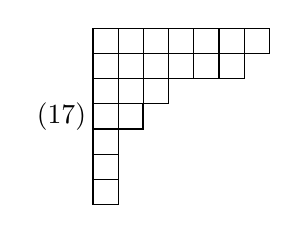
\begin{tikzpicture}[x=0.32cm,y=0.32cm]
\node at (-1.25,-3.5) {$(17)$};
\draw (0,0)--(7,0)--(7,-1)--(6,-1)--(6,-2)--(3,-2)--(3,-3)--(2,-3)--(2,-4)--(1,-4)--(1,-7)--(0,-7)--(0,0);
\draw (0,-1)--(6,-1) (0,-2)--(3,-2) (0,-3)--(2,-3) (0,-4)--(1,-4) (0,-5)--(1,-5) (0,-6)--(1,-6);
\draw (1,0)--(1,-4) (2,0)--(2,-3) (3,0)--(3,-2) (4,0)--(4,-2) (5,0)--(5,-2) (6,0)--(6,-1);
\draw[line width=0.8pt] (0,-4)--(2,-4)--(2,-3);
\end{tikzpicture}
\end{adjustbox}

Числа от $1$ до $n$ пишем в диаграмму — получ.
— станд таблица.

Каждое $k$ приобретает
\begin{adjustbox}{max width=\linewidth}
\begin{tikzpicture}[baseline=(ik.base)]
\node (ik) at (0,0) {$i_k$};
\node at (0.8,0) {и};
\node at (1.6,0) {$j_k$};
\draw (0,-0.25)--(0,-0.45);
\draw (1.7,-0.25)--(2.3,-0.4);
\node at (0,-0.75) {номер строки};
\node at (2.8,-0.75) {номер столбца};
\end{tikzpicture}
\end{adjustbox}
\begin{equation*}
u_k=i_k-j_k,\qquad u_1=0
\end{equation*}
Опред. жирной точки в (16).

У матриц разные кольца коэффициентов. При перемножении их берём
в элементах матриц
\begin{equation*}
A\bullet B=A\otimes B
\end{equation*}
$\mathcal{P}_\mu$ действует только на матричные коэффициенты
($\mathcal{P}_\mu$ — скалярная матрица)
\begin{equation*}
\mathcal{P}_\mu=\mathcal{P}_\mu 1
\end{equation*}
[У первого $\mathcal{P}_\mu$ зачёркнута надстрочная запись:
\Unclear{GELFAND-P001289}{projector-cancelled-superscript}{неразборчиво}.]

\underline{опред.}
\begin{equation*}
\mathcal{P}_\mu\in M_N^{\otimes n}
\end{equation*}
$\mathcal{P}_\mu$ — симметризатор по строкам и антисимм. по столбцам

На $M_N^{\otimes n}$ действует симм. группа $S_n$
\Unclear{GELFAND-P001289}{symmetric-group-order}{пор. $n$}

\SourcePage{GELFAND-P001290}{unlabelled}
\underline{5/V–86 г.}\qquad \underline{Г. Ольшанский.}
\underline{Бесконечномерные предст. и янгиан.}

(сем. Гельфанда)

$o(n)$ — компл. кососимм. матрицы $n\times n$
\begin{equation*}
o(\infty)=\bigcup_{n=1}^{\infty}o(n),
\end{equation*}
$\rho$ — тавтологич. предст. $o(\infty)$, действ. в
$\ell_2=\begin{pmatrix}a_1\\a_2\\\vdots\end{pmatrix}=H$
\begin{equation*}
\rho^{\otimes k}=\underbrace{\rho\otimes\cdots\otimes\rho}_{k\ \text{раз}},
\end{equation*}
[Справа зачёркнуто:
\Unclear{GELFAND-P001290}{rho-cancelled-mark}{неразборчиво}.]

\begin{equation*}
A=\Bigl\{X=(X_n),\ X_n\in U(o(n))
\end{equation*}
[Под $U$:] унив. обёрт. алг.
[Рядом зачёркнуто:
\Unclear{GELFAND-P001290}{enveloping-cancelled-mark}{неразборчиво}.]

\underline{св-ва}

1) сходимость:
$\exists\,s\text{-}\lim\limits_{n\to\infty}\rho^{\otimes k}(X_n)$
в $H^{\otimes k}$, $\forall k$
(предел обозначается $\rho^{\otimes k}(X)$)

2) конст.\qquad $\exists M=M(X):\ \operatorname{deg} X_n\le M$

3) конечн. индек:\qquad
$\exists m=m(X):\ X_n\in U(o(n))^{O_m(n)}$

$O_m(n)=$
\begin{adjustbox}{max width=\linewidth}
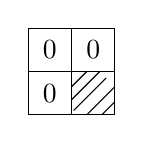
\begin{tikzpicture}[x=0.55cm,y=0.55cm,baseline=-0.6cm]
\draw (0,0) rectangle (2,-2);
\draw (1,0)--(1,-2) (0,-1)--(2,-1);
\node at (0.5,-0.5) {$0$};
\node at (1.5,-0.5) {$0$};
\node at (0.5,-1.5) {$0$};
\draw (1,-1.35)--(1.35,-1) (1,-1.65)--(1.65,-1) (1.05,-1.9)--(1.8,-1.15) (1.35,-2)--(2,-1.35) (1.7,-2)--(2,-1.7);
\end{tikzpicture}
\end{adjustbox}
$\simeq o(n-m)\Bigr\}$

[На левом поле перед теоремой перечёркнут знак:
\Unclear{GELFAND-P001290}{theorem-margin-mark}{неразборчиво}.]
\underline{Теорема.}
\begin{equation*}
A=\mathbb{C}[x_1,x_2,\ldots]\otimes Y,
\end{equation*}
где $Y$ — алг. с образ. $t_{ij}^{(M)}$, $M,i,j=1,2,\ldots$
\begin{equation*}
\begin{aligned}
(1)\quad &[t_{ij}^{(M+1)},t_{k\ell}^{(N)}]-[t_{ij}^{(M)},t_{k\ell}^{(N+1)}]\\
&=t_{kj}^{(M)}t_{i\ell}^{(N)}-t_{kj}^{(N)}t_{i\ell}^{(M)}
\end{aligned}
\end{equation*}
\underline{Замечание:} $Y$ — янгиан
[сверху приписано и соединено с этим словом:] (для $gl(n)$).
Фактически это
\Unclear{GELFAND-P001290}{yangian-realization-word}{опер. / очер.}
реализ. янгиана.

4)-е св-во:
Последовательности с одинаковыми пределами во всех представлениях
отождествляются:
\begin{equation*}
X\sim Y,\quad\text{если}\quad\rho^{\otimes k}(X)=\rho^{\otimes k}(Y)
\end{equation*}

$m=0\quad\Rightarrow\quad$ 3) выделяет центр

$m=1\quad\Rightarrow\quad$ 3)
[зачёркнуто:
\Unclear{GELFAND-P001290}{m-one-cancelled-mark}{неразборчиво}]
матр., коммут. с
\begin{adjustbox}{max width=\linewidth}
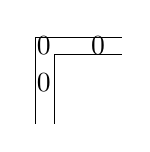
\begin{tikzpicture}[x=0.55cm,y=0.55cm,baseline=-0.4cm]
\draw (0,-2)--(0,0)--(2,0);
\draw (0.45,-2)--(0.45,-0.4)--(2,-0.4);
\node at (0.2,-0.2) {$0$};
\node at (1.45,-0.2) {$0$};
\node at (0.2,-1.05) {$0$};
\end{tikzpicture}
\end{adjustbox}
— \underline{зад. лин. алгебры.}

$Y=\bigcup Y_m$\qquad Можно фиксировать $m$.

$m$ фиксировано $\Rightarrow$ получается
\begin{equation*}
A_m=\mathbb{C}[x_1,x_2,\ldots]\otimes Y_m
\end{equation*}
\begin{equation*}
t_{ij}^{(M)}\qquad (i,j\le m;\ M=1,2,\ldots)
\end{equation*}

\SourcePage{GELFAND-P001291}{63}
Для $sp(\infty)$ получается та же $A$

Для $u(\infty)$ — || — $A\otimes A$.

Таким образом, всюду возникает одна и та же $A$ и это имеет
объяснение [зачёркнуто:
\Unclear{GELFAND-P001291}{explanation-cancelled-word}{неразборчиво}]
из теории представлений.

\underline{Предложение} И.М.Г.: рассмотреть такие случаи $m=0$, $m=1$

\underline{5/V–86 г.}\qquad \underline{\underline{Чередник И.}}

\begin{equation*}
1,\ 1^{ij}\in M_N,\qquad e_{ij}\in U(gl_N);\qquad
M_N\text{ — матрицы }N\times N;
\end{equation*}
\begin{equation*}
L(\lambda)=1+\frac{1}{\lambda}\sum_{i,j}e_{ij}1^{ji}
\in M_N(U(gl_N));
\end{equation*}
\begin{equation*}
H(\lambda)=\det_Q L(\lambda);
\end{equation*}
(см. опр. ниже)\qquad ($Q$ от слова \underline{quantum})

\begin{equation*}
\rho:gl_N\longrightarrow\operatorname{End}V\simeq M_d
\qquad (\text{предст.});
\end{equation*}
\begin{equation*}
L_V=1+\frac{1}{\lambda}\sum_{i,j}\rho(e_{ij})1^{ji}
\in M_N(\operatorname{End}V).
\end{equation*}
Пусть $V$ — предст. со [зачёркнут знак:
\Unclear{GELFAND-P001291}{weight-cancelled-mark}{неразборчиво}]
старшим весом
$\mu=(m_1,\ldots,m_\tau,0,\ldots,0)$
\begin{equation*}
m_1\ge m_2\ge\cdots\ge0,\qquad \tau\le N,\qquad m_j\in\mathbb{Z}_+
\end{equation*}
\begin{equation*}
V=V_\mu
\end{equation*}
Для группы:
\Unclear{GELFAND-P001291}{invariant-vector-uniqueness}{$\exists!$ вектор},
инвар. относит.
\begin{equation*}
\begin{pmatrix}
1&&\\
&\ddots&\\
0&&1
\end{pmatrix}
\end{equation*}
Тогда для
\SourceFigure{GELFAND-P001291}{triangular-matrix-last-entry}{Матрица в круглых скобках: $\lambda_1$ сверху слева, точки по диагонали, $0$ снизу слева, $\lambda$ с неясным малым знаком справа снизу; верхняя правая часть не заполнена.}
он соб. с [зачёркнут знак:
\Unclear{GELFAND-P001291}{eigenvalue-cancelled-mark}{неразборчиво}]
соб. знач. $\lambda_1^{m_1}\lambda_2^{m_2}\cdots\lambda_\tau^{m_\tau}$

и обязат. $m_1\ge m_2\ge\cdots\ge m_\tau$.

По нему однозн.
\Unclear{GELFAND-P001291}{reconstruction-abbreviation}{восстанавл. / восстановл.}
как?

Конструкция: с пом.
\begin{adjustbox}{max width=\linewidth}
\begin{tikzpicture}[baseline=(res.base)]
\node[inner sep=0pt] (res) at (0,0) {резольвент};
\draw (-0.85,-0.15)--(0.85,-0.15);
\node at (0.4,-0.5) {Б.Г.Г.};
\draw[rounded corners=9pt] (-0.35,-0.15)--(1.0,-0.15)--(1.0,-0.78)--(-0.35,-0.78)--(-0.35,-0.15);
\end{tikzpicture}
\end{adjustbox}
и т.д.

\underline{Опр. $H(\lambda)$:}
\begin{equation*}
\begin{aligned}
(1)\quad H(\lambda)\mathcal{P}_{-}^{N}
&=\mathcal{P}_{-}^{N}\bigl(L(\lambda+N-1)\otimes\cdots\otimes L(\lambda)\bigr)
\mathcal{P}_{-}^{N},\\
&H(\lambda)\in U(gl_N)
\end{aligned}
\end{equation*}
[Над тензорным произведением проведена скобка с подписью
$\in M_N^{\otimes N}(U(gl_N))$.]

(2) \underline{Теор.}
\begin{equation*}
H(\lambda)\big|_{V_\mu}\overset{\mathrm{def}}{=}
\det_Q L_{V_\mu}
=\prod_{i=1}^{\tau}\frac{\lambda+N+m_i-i}{\lambda+N-i}
\end{equation*}
(в частности, утверждается, что это скалярная ф-я)

$\mathcal{P}_{-}^{N}$ — антисимметризатор:
\begin{equation*}
\mathcal{P}_{-}^{N}(x_1\otimes\cdots\otimes x_N)
=\frac{1}{N!}\sum_{\sigma\in S_N}(-1)^{\epsilon(\sigma)}
(x_{\sigma(1)}\otimes\cdots\otimes x_{\sigma(N)}),
\qquad x_j\in\mathbb{C}^N
\end{equation*}
\SourceFigure{GELFAND-P001291}{antisymmetrizer-argument-annotation}{Под аргументом $x_1\otimes\cdots\otimes x_N$ расположен вертикальный знак с верхней дугой и тремя нижними штрихами, а под ним — $(\mathbb{C}^N)^{\otimes N}$; знак похож на повёрнутое $\in$ либо стрелку вверх.}

\SourcePage{GELFAND-P001292}{unlabelled}
\begin{equation*}
\mathcal{P}_{-}^{N}\in M_N^{\otimes N}
=\operatorname{End}\bigl((\mathbb{C}^{N})^{\otimes N}\bigr)
\end{equation*}
Образ $\mathcal{P}_{-}^{N}$ — одномерное подпр-во.

Справа в (1) — ограничение $L(\lambda+N-1)\otimes\cdots\otimes L(\lambda)$ на $1$-мерное подпр-во.

\begin{equation*}
H\mathcal{P}_{-}^{2}=\mathcal{P}_{-}^{2}(A\otimes B)\mathcal{P}_{-}^{2}
\qquad
\underbrace{\frac{1}{4}\bigl(a_{11}b_{22}+a_{22}b_{11}-a_{12}b_{21}-a_{21}b_{12}\bigr)}
\end{equation*}
[При продолжении этой строки перед дробью и справа от неё исправления:
\Unclear{GELFAND-P001292}{upper-coefficient}{перед $\frac{1}{4}$ зачёркнут знак, возможно $=$; справа от дроби затёртый штрих}.]
[После $a_{22}b_{11}$ зачёркнуто:
\Unclear{GELFAND-P001292}{upper-second-term-cancel}{$\frac{1}{2}$?}.]
[В последнем слагаемом перед $a_{21}$ зачёркнуто:
\Unclear{GELFAND-P001292}{upper-fourth-term-cancel}{$b_{12}$?; между $a_{21}$ и $b_{12}$ зачёркнуто $\frac{1}{2}$?}.]

[Под скобкой:] $H$ в случае, когда стоят произвольные матрицы.

\begin{equation*}
A=\begin{pmatrix}a_{11}&a_{12}\\a_{21}&a_{22}\end{pmatrix},
\qquad B=\begin{pmatrix}b_{11}&b_{12}\\b_{21}&b_{22}\end{pmatrix}.
\end{equation*}
\begin{equation*}
\begin{aligned}
a_{11}&=1+\frac{1}{\lambda+1}e_{11},&
a_{12}&=\frac{1}{\lambda+1}e_{21},\\
a_{22}&=1+\frac{1}{\lambda+1}e_{22},&
a_{21}&=\frac{1}{\lambda+1}e_{12}.
\end{aligned}
\end{equation*}
[Буква перед индексом $21$ во второй строке исправлена:
\Unclear{GELFAND-P001292}{middle-a21-correction}{$a_{21}$; прежняя буква неразборчива}.]
\begin{equation*}
\begin{aligned}
b_{11}&=1+\frac{1}{\lambda}e_{11},&
b_{12}&=\frac{1}{\lambda}e_{21},\\
b_{22}&=1+\frac{1}{\lambda}e_{22},&
b_{21}&=\frac{1}{\lambda}e_{12}.
\end{aligned}
\end{equation*}

\begin{equation*}
\begin{aligned}
H(\lambda)={}&\left(1+\frac{1}{\lambda+1}e_{11}\right)
\left(1+\frac{1}{\lambda}e_{22}\right)
+\left(1+\frac{1}{\lambda+1}e_{22}\right)
\left(1+\frac{1}{\lambda}e_{11}\right)-\\
&-\left(\frac{1}{\lambda+1}e_{12}\right)
\left(\frac{1}{\lambda}e_{21}\right)
-\left(\frac{1}{\lambda+1}e_{21}\right)
\left(\frac{1}{\lambda}e_{12}\right).
\end{aligned}
\end{equation*}
[В конце первой строки перед знаком минус зачёркнуто:
\Unclear{GELFAND-P001292}{lower-expansion-cancel}{$e$ с индексами; возможно $e_{11}$ или $e_{22}$}.]

\underline{Утв.:} $H(\lambda)$ на $\forall$ неприв. предст. кратен $1$
($\in$ центру).

[Зачёркнуто:
\Unclear{GELFAND-P001292}{lower-heading-cancel}{неразборчиво}.]
\Unclear{GELFAND-P001292}{lower-heading-abbreviation}{\underline{Пр. часть:}}
(Г. Ольшанский)

\begin{equation*}
\begin{aligned}
H(\lambda)={}&\sum\operatorname{sgn}
\begin{pmatrix}i_1&\cdots&i_N\\j_1&\cdots&j_N\end{pmatrix}
\left(\delta_{i_1j_1}+\frac{1}{\lambda+N-1}e_{i_1j_1}\right)\\
&\left(\delta_{i_2j_2}+\frac{1}{\lambda+N-2}e_{i_2j_2}\right)
\cdots\left(\delta_{i_Nj_N}+\frac{1}{\lambda}e_{i_Nj_N}\right)
\end{aligned}
\end{equation*}
[В знаменателе последнего множителя перед $\lambda$ зачёркнуто:
\Unclear{GELFAND-P001292}{lower-last-denominator-cancel}{неразборчивые знаки}.]

Если буквы $e_{ij}$ коммутируют (введем $h$) $\Rightarrow$ получится характ. многочлен.

Если некоммутир. — то это правильный аналог характ. многочлена.

Коммутируют: $\sum e_{ii}$, $\sum e_{ij}e_{ji}$ и т. д.


\SourcePage{GELFAND-P001293}{unlabelled}
% Review coordinates: source pixels [x0,y0,x1,y1), origin top-left; original 2432 x 3448.
% Originals inspected directly at full source resolution; listed crops enlarged for inspection.
% Review crop: header [220, 915, 1020, 1040]; scale=3x.
% Review crop: opening [240, 1030, 2100, 1180]; scale=2x.
% Review crop: agenda [125, 1180, 1240, 1440]; scale=3x.
% Review crop: introduction [230, 1440, 1870, 1825]; scale=2x.
% Review crop: closure-definition [210, 1790, 2335, 2070]; scale=2x.
% Review crop: axioms-cancelled [200, 2030, 2260, 2325]; scale=2x.
% Review crop: example [240, 2320, 1900, 2840]; scale=2x.
% Review crop: bottom [230, 2815, 2400, 3410]; scale=2x.
% Review crop: agenda-symbol [520, 1190, 615, 1265]; scale=8x.
% Review crop: cancel-b [302, 2060, 485, 2160]; scale=6x.
% Review crop: cancel-c-left [205, 2155, 825, 2330]; scale=4x.
% Review crop: cancel-c-middle [815, 2160, 1580, 2330]; scale=3x.
% Review crop: cancel-c-right [1560, 2160, 2260, 2330]; scale=3x.
% Review crop: theorem-names [235, 3020, 1550, 3165]; scale=3x.
% Review crop: strata-line-left [225, 3100, 1500, 3255]; scale=3x.
% Review crop: strata-line-right [1455, 3100, 2400, 3260]; scale=3x.
% Review crop: last-line [240, 3300, 1700, 3410]; scale=3x.
% Review crop: last-word [750, 3315, 1060, 3385]; scale=7x.
% Review crop: quadratic-word [750, 1240, 1160, 1345]; scale=4x.
% Review crop: closure-axiom-a [300, 1910, 755, 2025]; scale=4x.
% Review crop: closure-axiom-c [800, 2050, 1985, 2205]; scale=3x.
% Review crop: nondegenerate [235, 2800, 1755, 2950]; scale=3x.
% Review crop: example-first-index [1510, 2390, 1640, 2470]; scale=7x.
% Review crop: agenda [125, 1180, 1240, 1440]; scale=3x.
% Review crop: agenda-symbol [520, 1190, 615, 1265]; scale=8x.
% Review crop: theorem-names [235, 3020, 1550, 3165]; scale=3x.
% Review crop: strata-line-left [225, 3100, 1500, 3255]; scale=3x.
% Review crop: last-line [240, 3300, 1700, 3410]; scale=3x.
% Review crop: last-word [750, 3315, 1060, 3385]; scale=7x.

\underline{\underline{1/$\overline{\underline{\mathrm{IX}}}$ - 86 г.}}\qquad
\underline{Сем. Гельфанда.}

В Принстоне Виттен читал курс по \underline{струнам} и у него было 2 слушателя:
Делинь и Каждан.
[«струнам» подчёркнуто волнистой линией.]

\underline{И.М.Г. и Серганова}
\Unclear{GELFAND-P001293}{agenda-symbol}{[стрелка вправо; под ней неясный знак: двоеточие или зачёркнутый штрих]}
матроиды

\underline{Бейлинсон и Гинзбург:} квадр. алгебры

\underline{Чередник:} базис Гельфанда - Цейтлина

[Имена в трёх строках выше подчёркнуты волнистыми линиями.
На левом поле — прерывистая вертикальная черта.]

\underline{И.М. Гельфанд} (\underline{и Серганова}).

\underline{Общее определение матроида.}
[Волнистое подчёркивание.]

Гомологич. алгебра — раздел комбинаторики

В книге \underline{Айгнера} "Комбинат. теория" треть посвящена матроидам.
[«Айгнера» подчёркнуто волнистой линией.]

\underline{Опред. 1.}\qquad \underline{Матроид}.

Конечное мн-во и на нём понятие "замыкания":
$A\rightsquigarrow\bar A\supset A$, так что

а) \Unclear{GELFAND-P001293}{closure-axiom-a}{$\overline{A\cap B}=\bar A\cap\bar B$}
\qquad (но для $A\cup B$ не требуется)

б) [Зачёркнуто:
\Unclear{GELFAND-P001293}{cancel-b}{$a\in A$ или $a\in\bar A$; штрихи перекрыты зачёркиванием}.]
$\bar{\bar A}=\bar A$

[Справа, над зачёркнутой строкой, вписано:]
в) $a\notin\bar A,\ a\in\overline{A+\{b\}}
\Rightarrow b\in\overline{A+\{a\}}$

[Зачёркнуто: в)
\Unclear{GELFAND-P001293}{cancel-c-left}{$a\in\bar A,\ b\notin\bar A$; знаки принадлежности перекрыты штрихами}
$\{a\in A,\ b\in\bar A,\ b\ne a\}
\Rightarrow a\in\overline{A\setminus\{b\}}$.]

\underline{Пример}. В $R^n$ рассм. $k$ векторов $e_1,\ldots,e_k$
\begin{gather*}
A\subset\{1,2,\ldots,k\};\\
\bar A\ni i\ \Leftrightarrow\ e_i\in\text{лин. обол. }\{e_j,\ j\in A\}
\end{gather*}
\Unclear{GELFAND-P001293}{singleton-closure}{$\bar e_i=e_i$};
но $\overline{e_i\cup e_j}\ne\bar e_i\cup\bar e_j$ (вообще говоря).

\underline{Невыр. матроид} (или комбинат. геометрия): если $\bar\varnothing=\varnothing$.
[«Невыр. матроид» подчёркнуто волнистой линией.]

Где возникает матроид?

\underline{Теор.} (Гельф., Серг.,
\Unclear{GELFAND-P001293}{theorem-surname}{Горецки или Горески}, Макферсон).
Грассманово мн-ие
разбит
на страты (по действ. карт. подгруппы), есть и клетки Шуберта

В $R^n$ действ. диаг. матр. $\Rightarrow$ действ. на грассм.

Орбиты разбив. на
похожие
— это и есть страты.

\SourcePage{GELFAND-P001294}{71}
% Review coordinates: source pixels [x0,y0,x1,y1), origin top-left; original 2432 x 3448.
% Originals inspected directly at full source resolution; listed crops enlarged for inspection.
% Review crop: top [75, 25, 1220, 585]; scale=3x.
% Review crop: strip1 [130, 65, 2250, 635]; scale=3x.
% Review crop: strip2 [130, 600, 2280, 1050]; scale=3x.
% Review crop: strip3 [130, 1040, 2240, 1370]; scale=3x.
% Review crop: strip4 [120, 1360, 2210, 1790]; scale=3x.
% Review crop: strip5 [130, 1770, 1900, 2220]; scale=3x.
% Review crop: strip6 [130, 2180, 2200, 2610]; scale=3x.
% Review crop: strip7 [140, 2590, 2370, 2990]; scale=3x.
% Review crop: strip8 [100, 2970, 2390, 3440]; scale=3x.
% Review crop: topword [405, 75, 555, 173]; scale=6x.
% Review crop: voobsche [155, 900, 415, 1035]; scale=6x.
% Review crop: substitutions [575, 1035, 975, 1155]; scale=6x.
% Review crop: cancelshort [515, 1138, 640, 1220]; scale=10x.
% Review crop: rotationcomma [192, 1690, 580, 1810]; scale=6x.
% Review crop: reference [135, 2140, 1230, 2250]; scale=3x.
% Review crop: heading [160, 2535, 790, 2660]; scale=3x.
% Review crop: minimal [690, 2735, 1520, 2865]; scale=3x.
% Review crop: dittomarks [690, 2825, 1160, 2950]; scale=6x.
% Review crop: retracea [1020, 2625, 1165, 2730]; scale=6x.
% Review crop: retraceb [295, 2995, 410, 3120]; scale=6x.
% Review crop: refchapter [390, 2150, 575, 2230]; scale=6x.
% Review crop: coxname [620, 322, 845, 418]; scale=6x.
% Review crop: m12 [835, 725, 970, 785]; scale=10x.
% Review crop: curve [95, 2080, 290, 2360]; scale=3x.
% Review crop: bottomflag [1710, 3120, 2240, 3260]; scale=3x.
% Review crop: convextext [205, 2330, 1110, 2455]; scale=3x.
% Review crop: reviewer-brow [1100, 2830, 1780, 2990]; scale=5x.

Каждый страт в $G_{n,k}$ однозначно задаётся матроидом.

\underline{Общее опр. матроида}

Пусть дана гр. Кокстера, порожд. $s_1,\ldots,s_n$

(т. е. есть соотн. $s_i^2=1$, $(s_i s_j)^{m_{ij}}=1$,

$m_{ij}$ — зад. целочисл. матрица)

\underline{Прим.}

А. $1,s_1$ — 2 элемента

Б. $1,s_1,s_2$ —
\Unclear{GELFAND-P001294}{two-generator-finiteness}{$(s_1s_2)^{m_{12}}=1$ \quad Гр. уже может быть бесконечна!}

Вопрос: когда? (для первокурсников)

\Unclear{GELFAND-P001294}{voobsche-edit}{Вообще: [статус правки неясен]}
Когда конечна? Уже трудно.

\underline{Пример:} [волнистое подчёркивание]
гр. \Unclear{GELFAND-P001294}{permutation-noun}{подстановок}
$S_n$ из $n$ элементов;

$s_j$ — \Unclear{GELFAND-P001294}{cancelled-short-word}{[зачёркнуто: это?]}
перестан. 2-х элементов (соседних). ($j$ и $j+1$)

\begin{equation*}
(s_i s_{i+1})^3=1,\qquad (s_i s_k)^2=1
\quad\text{при несоседних }i\text{ и }k.
\end{equation*}

$H^3$: $s_1,s_2,s_3$:

\begin{equation*}
(s_1s_2)^5=1,\qquad (s_2s_3)^3=1,\qquad (s_1s_3)^2=1
\qquad\text{(120 элементов)}
\end{equation*}

(гр. симметрий икосаэдра!)

[Между строками: или додекаэдра:]

\Unclear{GELFAND-P001294}{rotation-generator-separator}{$s_1,s_2$ — вращ. вокруг вершины}

\begin{center}
\begin{adjustbox}{max width=\linewidth}
\begin{tikzcd}[row sep=large,column sep=large]
SU(2)=S^3 \arrow[r,"{\text{2-лист. накр.}}"'] & SO(3) & \\
120 \arrow[u,phantom,"\cup" description] \arrow[r] &
60 \arrow[u,phantom,"\cup" description] & \text{— вращения икосаэдра}
\end{tikzcd}
\end{adjustbox}
\end{center}

(См. 1-ю гл. кн. Гельф. — Минлос — Шапиро)

\SourceFigure{GELFAND-P001294}{rotation-margin-arrow}{Слева от справочной строки видны два раздельных изогнутых участка: верхний начинается под числом $120$ в схеме и огибает открывающую скобку; нижний оканчивается стрелкой вправо-вниз перед словами «120 точек». Непрерывность соединения участков неясна.}

$120$ точек в $S^3=SU(2)$

Вып. оболочка — прав. многр.; имеющий $600$ граней — тетраэдров

Его гр. симметрий $H^4$: $120^2$ — её порядок.

\underline{Флаговый} \underline{матроид.}

Пусть есть гр. Кокстера; $a=s_{i_1}\ldots s_{i_\ell}$
пусть запись минимальна (самая короткая)

$a<b$, если $\exists\min$ разл. $a=w_{i_1}\ldots w_{i_\ell}$

$\exists$ \SourceFigure{GELFAND-P001294}{bruhat-ditto}{После второго знака существования написаны длинная горизонтальная черта, два коротких наклонных штриха и ещё одна длинная черта; буквенная расшифровка знака повтора не добавлена.}
$b=.\,.\,.\,.(w_{i_1}\ldots w_{i_\ell})\ldots$.

(упорядочение Брюа)

$a\overset{w}{<}b$, если $w^{-1}a<w^{-1}b$

$W$ — гр. Кокстера, $L\subset W$, $\operatorname{Card}L<\infty$.
$L$ наз. \underline{флаг. матроидом} [волнистое подчёркивание], если

$\forall$ $w$-упорядочения в $L$ есть $\min$ элемент.

Можно перечислить все конечные гр. Кокстера и соотв. матроиды.

\SourcePage{GELFAND-P001295}{unlabelled}
% Review coordinates: source pixels [x0,y0,x1,y1), origin top-left; original 2432 x 3448.
% Originals inspected directly at full source resolution; listed crops enlarged for inspection.
% Review crop: top-heading-left [220, 20, 1270, 235]; scale=3x.
% Review crop: top-heading-right [1200, 20, 2280, 220]; scale=3x.
% Review crop: cancelled-box-left [200, 255, 1230, 455]; scale=3x.
% Review crop: cancelled-box-right [1200, 255, 2370, 455]; scale=3x.
% Review crop: question-diagram [205, 450, 1655, 942]; scale=3x.
% Review crop: section-heading [220, 942, 1840, 1067]; scale=3x.
% Review crop: algebra-lines [220, 1065, 2280, 1335]; scale=3x.
% Review crop: relations [235, 1300, 1150, 1430]; scale=3x.
% Review crop: example-requirement [230, 1410, 2010, 1685]; scale=3x.
% Review crop: tensor [245, 1650, 1740, 1920]; scale=3x.
% Review crop: required-relation [170, 1910, 2250, 2245]; scale=3x.
% Review crop: dual [210, 2240, 2100, 2640]; scale=3x.
% Review crop: example-bottom [250, 2645, 2250, 3150]; scale=3x.
% Review crop: diagram-detail [230, 630, 580, 925]; scale=5x.
% Review crop: cancelled-box-word [465, 267, 590, 400]; scale=5x.
% Review crop: cancelled-relations-word [285, 1315, 505, 1430]; scale=8x.
% Review crop: cancelled-a0-word [402, 1157, 690, 1234]; scale=6x.
% Review crop: grading-word [859, 1068, 1168, 1160]; scale=5x.
% Review crop: tensor-cancelled-superscript [1060, 1760, 1260, 1880]; scale=6x.
% Review crop: dual-full-tensor [235, 2133, 1540, 2300]; scale=3x.
% Review crop: ideal-glyphs [1010, 2030, 2220, 2230]; scale=4x.
% Review crop: bottom-indices [310, 2760, 1390, 2900]; scale=4x.
% Review crop: heading-work [239, 953, 1720, 1075]; scale=4x.
% Review crop: bottom-first-index [444, 2780, 556, 2895]; scale=10x.
% Review crop: bottom-second-index [552, 2780, 668, 2895]; scale=10x.
% Review crop: relations-cancelled-full [256, 1288, 990, 1445]; scale=5x.
% Review crop: title-abbrev [925, 40, 1235, 165]; scale=6x.
% Review crop: a0-cancelled-wide [300, 1125, 847, 1264]; scale=5x.
% Review crop: example-abbreviation [1315, 1418, 1885, 1533]; scale=5x.
% Review crop: subspace-label [246, 1663, 572, 1820]; scale=4x.
% Review crop: graded-line-left [218, 1060, 876, 1179]; scale=4x.
% Review crop: requirements-line-left [165, 1912, 897, 2070]; scale=4x.
% Review crop: ideal-definition [1370, 2020, 2230, 2240]; scale=5x.
% Review crop: bottom-relation-line [243, 2900, 1487, 3067]; scale=3x.
% Review crop: margin-rule-final [45, 1260, 235, 1790]; scale=3x.
% Review crop: diagram [240, 630, 600, 930]; scale=5x.
% Review crop: bottom-index [444, 2780, 556, 2895]; scale=10x.
% Review crop: upper [65, 420, 2210, 1190]; scale=2x.
% Review crop: bottom [180, 2590, 2085, 3140]; scale=2x.
% Review crop: factor-row [342, 2765, 1370, 2910]; scale=4x.
% Review crop: n-reference [1960, 2660, 2110, 2780]; scale=8x.

Матроид из векторов полностью опред. списком $\max$ наборов лин. независ.\\
Векторов.
[Обе строки подчёркнуты волнистой линией.]

[В рамке; зачёркнуто: \underline{\underline{Опред.}}
\Unclear{GELFAND-P001295}{upper-cancelled-fragment}{неразборчиво}
Параб. подгруппа $P$ гр. Кокстера — это подгруппа, порожд.\\
мн-вом $S\ldots$]

Всякий ли матроид представим как векторный?

Не всякий!!

\SourceFigure{GELFAND-P001295}{seven-point-diagram}{Треугольный рисунок с семью отмеченными точками: 1 внизу слева, 2 на левой стороне, 3 в верхней вершине, 4 на правой стороне, 5 внизу справа, 6 на нижней стороне, 7 внутри. Видны стороны треугольника, внутренние прямые, прерывистые и кривые штрихи; точная форма и соединение части внутренних штрихов около 7 неясны.}
\begin{equation*}
\begin{array}{ccc}
1\,2\,3 & 2\,7\,5 & 2\,4\,6\\
1\,6\,5 & 1\,7\,4 & \\
3\,4\,5 & 3\,7\,6 &
\end{array}
\end{equation*}

\underline{\underline{О раб. Бейлинсона и Гинзбурга.}}
\underline{\underline{"Квадр. алгебры"}}.

Рассм. градуир. алгебра с целочисл. градуировкой $(0,1,2,\ldots\;\text{— степени})$

$A_0$ — [зачёркнуто: \Unclear{GELFAND-P001295}{cancelled-a0-word}{алгебра?}] поле;

Треб., чтобы алгебра порождалась $A_1=V$ $(\dim_{A_0}V<\infty)$.

[Зачёркнуто: \Unclear{GELFAND-P001295}{cancelled-before-relations}{Квадр. / Зад.?}] Соотношения?

[На левом поле рядом со строками о соотношениях — прерывистая вертикальная черта.]

\underline{Пример}: $x_i x_k-x_k x_i=0\quad\Rightarrow$ алг. многочленов.

\underline{Требование}: все соотн. порождаются элементами $V\otimes V$.
\begin{equation*}
\underset{\text{подпр-во.}}{W}\subset V\otimes V
\end{equation*}
[От $W$ к подписи проведён короткий вертикальный штрих.]
\begin{equation*}
A_0\oplus V\oplus(V\otimes V)\oplus\ldots\oplus V^{\otimes n}\oplus\ldots=T(V)
\end{equation*}
[После $V$, перед $\otimes n$, зачёркнут надстрочный знак:
\Unclear{GELFAND-P001295}{cancelled-tensor-exponent}{$n$?}.]

Требуется: $\exists$ лин. пр-во $W\subset V\otimes V$, порожд. все соотн. в $A$.
\begin{equation*}
\begin{gathered}
(A=T(V)/J,\quad\text{где }J\text{ порожд. }W\\
J=J(W))
\end{gathered}
\end{equation*}

Дуальная:
\begin{equation*}
A_0\oplus V^*\oplus V^*\otimes V^*\oplus\ldots\oplus(V^*)^{\otimes n}\oplus\ldots
\end{equation*}

Рассм. в ней $W^\perp\subset V^*\otimes V^*$ и соотв. алгебру
\begin{equation*}
A^!=T(V^*)/J(W^\perp).
\end{equation*}
Она наз. \underline{двойственной} алгеброй.
[Подчёркивание слова «двойственной» волнистое.]

\underline{Пример 1.} Пусть $A$ — коммут. алгебра \underline{многочленов} от $x_1,\ldots,x_n$
[Подчёркивание слова «многочленов» волнистое.]
\begin{center}
\Unclear{GELFAND-P001295}{lower-first-product-index}{$\bigl(x_i x_n-x_k x_i\bigr)\perp\bigl(x_i^*x_k^*+x_k^*x_i^*\bigr)$}
\end{center}

Соотнош.: $\sum a_{ij}\,x_i\otimes x_j$ с $a_{ij}=-a_{ji}$

$A^!$ — грассманова алгебра.

\SourcePage{GELFAND-P001296}{72}
% Review coordinates: source pixels [x0,y0,x1,y1), origin top-left; original 2432 x 3448.
% Originals inspected directly at full source resolution; listed crops enlarged for inspection.
% Review crop: top [110, 30, 2220, 385]; scale=3x.
% Review crop: example [230, 360, 1580, 604]; scale=3x.
% Review crop: middle [210, 575, 1830, 1180]; scale=3x.
% Review crop: relations [170, 1140, 1690, 1410]; scale=3x.
% Review crop: bottom [150, 1390, 1870, 1900]; scale=3x.
% Review crop: crossedtop [1400, 120, 1870, 275]; scale=3x.
% Review crop: crossedbottom [165, 1620, 790, 1750]; scale=3x.
% Review crop: ideal [665, 124, 973, 371]; scale=6x.
% Review crop: commut [1920, 52, 2179, 161]; scale=6x.
% Review crop: middle-index [361, 745, 803, 867]; scale=6x.
% Review crop: perp-cancel [1605, 966, 1794, 1090]; scale=6x.
% Review crop: bottom-indices [188, 1624, 761, 1730]; scale=6x.
% Review crop: bottom-known [857, 1620, 1332, 1744]; scale=6x.
% Review crop: top-qn [1290, 44, 1510, 194]; scale=6x.
% Review crop: perp-w [315, 917, 550, 1085]; scale=6x.
% Review crop: topline-left [132, 40, 1435, 236]; scale=4x.
% Review crop: perp-line [530, 917, 1540, 1120]; scale=4x.
% Review crop: trace-text [430, 1069, 1103, 1180]; scale=4x.
% Review crop: finalword [214, 1726, 783, 1868]; scale=4x.
% Review crop: label [2250, 35, 2380, 165]; scale=4x.
% Review crop: topcancel-detail [1430, 143, 1837, 250]; scale=4x.
% Review crop: ideal-top [482, 125, 750, 242]; scale=8x.

\underline{Пример 2.} Рассм. $n$ кв. форм: $Q_1,\ldots,Q_n$
[Подчёркивание «Пример 2.» прерывистое.]
[зачёркнуто: \Unclear{GELFAND-P001296}{top-qn-cancellation}{неразборчивый знак}]
и фактор всех коммут. многочленов по
\Unclear{GELFAND-P001296}{top-ideal-delimiters}{$J(Q)$ или $J\langle Q\rangle$}, т.е.

[Справа от второй строки зачёркнуто:
\Unclear{GELFAND-P001296}{top-parenthetical-cancellation}{(симм. билин. формы)}.]

[Над формулой справа:
\Unclear{GELFAND-P001296}{top-detached-tv}{$T(V)$}.]
\begin{gather*}
A=S(V)/J(Q)
\end{gather*}

\underline{Например:}
[Волнистое подчёркивание.]
\begin{equation*}
\sum x_i^2=0,\qquad
\begin{adjustbox}{max width=\linewidth}
\begin{tikzpicture}[baseline=(comm.base)]
\node[inner sep=0pt] (comm) {$x_ix_j-x_jx_i$};
\node[anchor=west,inner sep=0pt] at (comm.east) {$=0.$};
\draw ([yshift=-2pt]comm.south west) -- ++(0,-4pt) -| ([yshift=-2pt]comm.south east);
\node[anchor=north,inner sep=0pt,yshift=-8pt] at (comm.south) {на них натянуто $W_1$};
\end{tikzpicture}
\end{adjustbox}
\end{equation*}
$W$ натянуто на $W_1$ и $\sum x_i^2$

Их лин. комбинации ?
\begin{gather*}
\sum a_{ij}x_i x_k,\qquad
\begin{aligned}
a_{ij}&=-a_{ji},\quad i\ne j\\
a_{ii}&=a_{jj}
\end{aligned}
\end{gather*}
\Unclear{GELFAND-P001296}{middle-sum-index}{$k$ в $\sum a_{ij}x_i x_k$; соотношение индексов не выяснено.}

\begin{gather*}
W^\perp=\{b_{ij}x_i^*x_j^*;\quad b_{ij}=b_{ji};\quad \sum b_{ii}=0\}
\end{gather*}
[Справа: $($ и зачёркнуто:
\Unclear{GELFAND-P001296}{middle-parenthetical-cancellation}{неразборчивый знак}.]

симм. матр. со следом $0$.

\underline{Независимые соотношения:}
[Волнистое подчёркивание.]
\begin{gather*}
y_i y_j+y_j y_i=0\ \text{при }i\ne j;\qquad
y_i^2=y_j^2\quad(\forall i,j)
\end{gather*}

Положим $y_i^2=h$. Тогда
\begin{gather*}
y_i y_j+y_j y_i=2\delta_{ij}h.
\end{gather*}

[Слева зачёркнуто:
\Unclear{GELFAND-P001296}{lower-cancelled-equation}{$y_1y_2y_1+y_2y_1^2=0$}.]
\begin{gather*}
y_1^2y_i=y_i y_1^2\qquad(\text{т.к. }y_1^2=y_i^2)
\end{gather*}
$\Rightarrow\ h\in$ \underline{центру}!
[Волнистое подчёркивание.]



\end{document}
